%*******10********20********30********40********50********60********70********80

% For all chapters, use the newdefined chap{} instead of chapter{}
% This will make the text at the top-left of the page be the same as the chapter

\chap{Θεωρητικό Υπόβαθρο και Σχετική Βιβλιογραφία} \label{c:complex}
%ΠΕΡΙΓΡΑΦΗ ΤΟΥ ΤΙ ΑΚΡΙΒΩΣ ΠΑΡΟΥΣΙΑΖΕΤΑΙ ΣΤΟ ΚΕΦΑΛΑΙΟ

Στο συγκεκριμένο κεφάλαιο γίνεται επεξήγηση των βασικών εννοιών και τεχνολογιών που αναφέρονται στην εργασία. Παρουσιάζονται οι έννοιες της Επαυξημένης Πραγματικότητας, του μοντέλου κάμερας pinhole, της ανίχνευσης δεικτών (markers) και το πεδίο της αναγνώρισης χειρονομιών σε εφαρμογές. Επιπλέον γίνεται ανασκόπηση των σχετικών επιστημονικών εργασιών και εφαρμογών, καθώς και των ανοικτών προκλήσεων στον ερευνητικό τομέα.



\section{Επαυξημένη Πραγματικότητα}
%ΟΡΙΣΜΟΣ+ΤΙ ΥΠΑΡΧΕΙ ΣΗΜΕΡΑ+ΔΙΑΦΟΡΑ ΑΠΟ VR+ OTI EXEI NA KANEI ME AR APO ERGASIES ALLON


%verykokou
Ο όρος επαυξημένη πραγματικότητα, διεθνώς γνωστή ως augmented reality (AR), αναφέρεται στην τεχνολογία που επιτρέπει την προσθήκη ψηφιακών πληροφοριών, που παράγονται από έναν υπολογιστή, στον πραγματικό κόσμο, μέσω κατάλληλων συσκευών. Πρόκειται για ένα ταχέως εξελισσόμενο ερευνητικό πεδίο, το οποίο στοχεύει στον εμπλουτισμό της αντίληψης της πραγματικότητας από το χρήστη.


Ιδανικά, τα αντικείμενα που συμπληρώνουν τον πραγματικό κόσμο παρουσιάζονται να συνυπάρχουν στον ίδιο χώρο με αυτόν. Ωστόσο, δεν αποτελούν μόνο οπτικές πληροφορίες. Η επαυξημένη πραγματικότητα, δυνητικά, μπορεί να βελτιώσει και τις πέντε αισθήσεις, και κυρίως – εκτός από την όραση – την ακοή και την αφή, αν και σήμερα η κυρίαρχη χρήση της είναι η προσθήκη οπτικών πληροφοριών στον πραγματικό κόσμο. 


Υπάρχουν διάφοροι ορισμοί της επαυξημένης πραγματικότητας, εκ των οποίων ευρέως αποδεκτός είναι ο ορισμός που έδωσε ο Ronald Azuma το 1997 \cite{azuma1997}. Σύμφωνα με αυτόν, η επαυξημένη πραγματικότητα είναι μία παραλλαγή της εικονικής πραγματικότητας (virtual reality), αλλά δε θα πρέπει να συγχέεται με την τελευταία, διότι συμπληρώνει τον πραγματικό κόσμο και δεν τον υποκαθιστά. 



Στόχος της εικονικής πραγματικότητας είναι η πλήρης «εμβύθιση» του χρήστη σε ένα περιβάλλον πλήρως ελεγχόμενο από υπολογιστή, το οποίο δεν του επιτρέπει να δει τον πραγματικό κόσμο γύρω του. Οι χρήστες εμβυθίζονται σε μία σκηνή που αν και αποτελείται εξ' ολοκλήρου από γραφικά, γίνται αντιληπτή σαν να ήταν πραγματική.  Για να δημιουργηθεί μια ρεαλιστική εικονική σκηνή, το επίπεδο των λεπτομερειών των γραφικών που συνιστούν τα αντικείμενα της εικονικής σκηνής πρέπει να είναι ιδιαίτερα υψηλό και η απεικόνιση πρέπει να πραγματοποιείται σε πραγματικό χρόνο. Ωστόσο όσο υψηλότερο είναι το επίπεδο των λεπτομερειών, τόσο μειώνεται η απόδοση ενός συστήματος προσπαθώντας να τα απεικονίσει. Ο συνθετικός αυτός κόσμος μπορεί να μιμείται τις ιδιότητες ενός πραγματικού κόσμου, είτε αυτός υπάρχει είτε όχι, ή και να διαφέρει σημαντικά από την πραγματικότητα, δημιουργώντας ένα φανταστικό κόσμο, στον οποίο οι φυσικοί νόμοι δεν ισχύουν πλέον [8]. 


Η επαυξημένη πραγματικότητα στοχεύει στην ενσωμάτωση συνθετικών πληροφοριών στο πραγματικό περιβάλλον – ή σε ένα βίντεο του πραγματικού περιβάλλοντος – με αποτέλεσμα αυτό να μην αποκρύπτεται εντελώς, αλλά αντίθετα να έχει κυρίαρχο ρόλο. Τα εικονικά αντικείμενα σε ένα περιβάλλον επαυξημένης πραγματικότητας, δεν είναι απαραίτητο να έχουν ένα υψηλό επίπεδο λεπτομερειών. Η ρεαλιστική ποιότητά τους περιορίζεται μόνο από τις παραμέτρους της εφαρμογής. 

Μία ακόμα διαφορά ανάμεσα σε συστήματα επαυξημένης και εικονικής πραγματικότητας βασίζεται στο ποσοστό του περιεχομένου της σκηνής που απεικονίζεται. Ένα σύστημα επαυξημένης πραγματικότητας, στο οποίο απεικονίζονται μόνο μερικά απλά εικονικά αντικείμενα σε μία σκηνή, απαιτεί λιγότερη ισχύ από ένα σύστημα εικονικής πραγματικότητας, στο οποίο πρέπει να απεικονίζεται ολόκληρη η σκηνή.


Επιπλέον, διαφορές ανάμεσα στα δύο συστήματα παρατηρούνται στο πρόβλημα του registration(γεωαναφορά). Αφού το registration ασχολείται με τη σωστή τοποθέτηση εικονικών αντικειμένων εντός ενός πραγματικού περιβάλλοντος, τα συστήματα εικονικής πραγματικότητας δεν επηρεάζονται, αφού έχουν να κάνουν μόνο με εικονικές σκηνές. Η θέση όλων των αντικειμένων σε μία σκηνή VR περιγράφεται με βάση ένα κοινό σύστημα συντεταγμένων. Αυτό σημαίνει ότι ένα σύστημα VR έχει πάντα σωστό registration χωρίς να πρέπει να σπαταλά υπολογιστικούς πόρους για την εύρεσή του. Όσον αφορά την απόδοση, το χαμηλό υπολογιστικό κόστος για απεικόνιση γραφικών χαμηλής ποιότητας αντισταθμίζεται από το υπολογιστικό κόστος που απαιτείται για το registration.

Τέλος, στα συστήματα VR, οι συσκευές απεικόνισης χρησιμοποιούνται για να ανιχνεύουν τη τη θέση του χρήστη μαζί με μία οθόνη που απεικονίζει την ψηφιακή σκηνή. Σε ένα σύστημα επαυξημένης πραγματικότητας, υπάρχουν πολλοί διαφορετκοί συνδυασμοί εξοπλισμοί για την ανίχνευση και την πληροφόρηση του χρήστη.
%---

Τα συστήματα επαυξημένης πραγματικότητας σύμφωνα με την καταπληκτική ερευνητική επισκόπηση του πεδίου από τους Azuma et al. (2001) έχουν τα ακόλουθα τρία χαρακτηριστικά \cite{azuma2001}:

\begin{itemize}
\item Συνδυάζουν το πραγματική με την εικονική πληροφορία
\item Επιτρέπουν την αλληλεπίδραση σε πραγματικό χρόνο
\item Λειτουργούν αναφορικά με τον πραγματικό τρισδιάστατο κόσμο
\end{itemize}  


Τα παραπάνω χαρακτηριστικά καθίστανται σημαντικά στην αξιολόγηση αν ένα σύστημα είναι σύστημα επαυξημένης πραγματικότητας ή όχι. Έτσι, για παράδειγμα, κάποιες ταινίες, μολονότι μπορεί να περιλαμβάνουν φωτορεαλιστικά εικονικά αντικείμενα τα οποία συνδυάζονται ομαλά με το τρισδιάστατο πραγματικό περιβάλλον, δεν είναι διαδραστικές σε πραγματικό χρόνο και επομένως δεν αποτελούν συστήματα επαυξημένης πραγματικότητας \cite{azuma1997}. Αντίθετα, η εισαγωγή των εικονικών δεδομένων οφείλεται σε προεπεξεργασία, η οποία αντιτίθεται με το δεύτερο χαρακτηριστικό των συστημάτων επαυξημένης πραγματικότητας.

%augmented virtuality continuum
Σύμφωνα με τους Paul Milgram et al. (1994), η επαυξημένη πραγματικότητα ανήκει στην τεχνολογία της μικτής πραγματικότητας (mixed reality) [8].

Στη δημοσίευσή τους, ορίζεται το «συνεχές πραγματικότητας - εικονικότητας» (reality - virtuality continuum), το οποίο μπορεί να χρησιμοποιηθεί για τη σύγκριση των διαφόρων μορφών της μεικτής πραγματικότητας με την τοποθέτησή τους σε ένα φάσμα, όπως φαίνεται στην Εικόνα 1-1. 

Στη μία άκρη του φάσματους βρίσκεται το πραγματικό περιβάλλον, που δεν περιέχει καμία εικονική πληροφορία. Ενώ μετακινούμαστε προς τα δεξιά, εντοπίζεται η επαυξημένη πραγματικότητα, όπου τα τεχνητά αντικείμενα προστίθενται στον φυσικό κόσμο. Αμέσως πιο δεξιά, εντοπίζεται η επαυξημένη εικονικότητα, όπου τα αντικείμενα του φυσικού κόσμου(όπως μία ζωντανή απεικόνιση μίας απομακρυσμένης προβολής) προστίθενται σε ένα πλήρως εικονικό περιβάλλον "εμβύθισης". Φτάνοντας στο δεξί άκρος του φάσματος, παρατηρείται ένα πλήρως συνθετικό περιβάλλον, στο οποίο δεν υπάρχει καμία πληροφορία από τον φυσικό κόσμο.Κάθε είδος 3D περιβάλλοντος μπορεί να τοποθετηθεί κατά μήκος του φάσματος και μπορεί να χρησιμοποιηθεί για την εύκολη σύγκριση των χαρακτηριστικών του.

Επομένως στο περιβάλλον μεικτής πραγματικότητας, αντικείμενα του πραγματικού και του εικονικού κόσμου – δηλαδή οτιδήποτε μεταξύ των άκρων του συνεχούς – παρουσιάζονται μαζί σε μία συσκευή θέασης. Η μεικτή πραγματικότητα περιλαμβάνει τόσο την επαυξημένη πραγματικότητα, όσο και την επαυξημένη εικονικότητα (augmented virtuality). Ενώ στην πρώτη, το περιβάλλον που παρατηρείται είναι κυρίως αληθινό και έχουν προστεθεί βελτιώσεις που παράγονται από υπολογιστή, στην επαυξημένη εικονικότητα το παρατηρούμενο περιβάλλον είναι κυρίως εικονικό και επαυξάνεται με τη χρήση πραγματικών δεδομένων.

%ADD IMAGE OF CONTINUUM

Αυτός ο ορισμός δεν περιορίζει την επαυξημένη πραγματικότητα στη χρήση μόνο συσκευών απεικόνισης που τοποθετούνται στο κεφάλι του χρήστη(HMDs), επιτρέποντας τη χρήση προβολέων και φορητών συσκευών απεικόνισης, αλλά απκλείοντας μη διαδραστικά μέσα όπως οι ταινίες και τα τηλεοπτικά δρώμενα. 

Για να υπερθέσουμε τρισδιάστατα εικονικά μοντέλα σε αυτ΄που βλέπουν οι χρήστες, ένα σύστημα ΑR πρέπει να συνδυάζει τις πληροφορίες που παράγονται από έναν υπολογιστή με αισθητήρες που μπορούν να μετρήσουν τη θέση και τον προσανατολισμό του χρήστη. 

Καθώς ο χρήστης κινείται στο φυσικό κόσμο, η απεικόνιση των πληροφοριών ανανεώνεται σε πραγματικό χρόνο από τον υπολογιστή. Η ακρίβεια της τοποθέτησης των εικονικών αντικειμένων πάνω στο φυσικό κόσμο επηρεάζει τον ρεαλισμό της εμπειρίας του χρήστη.


%-----------


%AR=Combination of Computer Graphics & COmputer Vision
Ουσιαστικά η επαυξημένη πραγματικότητα αποτελεί συνδυασμό του κλάδου των Γραφικών Υπολογιστών και της Όρασης Υπολογιστών. Ο συνδυασμός αλγορίθμων και μεθόδων των δύο αυτών συγγενών επιστημών είναι το κλειδί για την επίτευξη σημαντικών αποτελεσμάτων σε εφαρμογές που επεξεργάζονται εικόνες ή βίντεο, εξάγουν πληροφορίες από μία σκηνή και επαυξάνουν τη σκηνή με γραφικά.

Για να μπορέσει ο υπολογιστής να δημιουργήσει συναφείς πληροφορίες, πρέπει πρώτα να κατανοήσει κάποιες παραμέτρους. Οι παράμετροι αυτοί έχουν να κάνουν με πληροφορίες σχετικά με το περιβάλλον στο οποίο βρίσκεται ο χρήστης, καθώς και με τη θέση και τον προσανατολισμό του μέσα στο περιβάλλον αυτό. Με βάση αυτές τις πληροφορίες, ο υπολογιστής μπορεί να τοποθετήσει τις επαυξημένες πληροφορίες σωστά σε σχέση με τoν περιβάλλοντα χώρο. Αυτή η εναρμόνιση των εικονικών αντικειμένων με αντικείμενα της πραγματικής σκηνή είναι γνωστή με τον όρο registration. 

Η ανάπτυξη των τεχνικών της όρασης υπολογιστών συντελεί στην καλύτερη αναγνώριση της σκηνής και την εξαγωγή χαρακτηριστικών που βοηθούν στη γνώση της ακριβούς τοποθεσίας στην οποία πρέπει να τοποθετηθούν τα εικονικά αντικείμενα. Ορισμένες ερευνητικές μέθοδοι που αναπτύχθηκαν στο πεδίο της όρασης υπολογιστών εφαρμόζονται και σε συστήματα επαυξημένης πραγματικότητας. Μερικές από αυτές είναι ο εντοπισμός και η ανίχνευση markers και χαρακτηριστικών μία σκηνής, η ανίχνευση και ο εντοπισμός κίνησης, η ανάλυση εικόνας, η αναγνώριση χειρονομιών και η κατασκευή περιβαλλόντων που περιέχουν έναν αριθμό από διαφορετικούς αισθητήρες.


Από την άλλη πλευρά, τα γραφικά συντελούν στην επαύξηση της πραγματικότητας με τη φωτορεαλιστική απεικόνιση τρισδιάστατων μοντέλων σε πραγματικό χρόνο, και τις διαδραστικές κινήσεις τους (animations)

%-------------------------------------------------


Ένα τυπικό σύστημα επαυξημένης πραγματικότητας μπορεί να διαιρεθεί σε 2 κύριες εργασίες: το tracking και το registration.
Πρέπει δηλαδή να ανιχνευθεί ένα γνωστό πρότυπο που είναι αποθηκευμένο στη μνήμη ενός υπολογιστή(marker tracking) \cite{krevelen2010} και έπειτα να προστεθεί ένα εικονικό αντικείμενο στη σκηνή σωστά πάνω σε αυτό το πρότυπο.



\subsection{Ιστορική Αναδρομή}
%ΣΥΝΤΟΜΗ ΙΣΤΟΡΙΚΗ ΑΝΑΔΡΟΜΗ ΑΠΟ ΑΛΛΕΣ ΕΡΓΑΣΙΕΣ

Η τεχνολογίας της επαυξημένης πραγματικότητας υπαινίσσεται για πρώτη φορά το 1901, μέσα από το μυθιστόρημά του Frank Baum με τίτλο «The Master Key», όπου περιγράφεται ένα ζευγάρι ειδικών γυαλιών, το οποίο υπερθέτει στο μέτωπο του κάθε ανθρώπου, που βρίσκεται στο οπτικό πεδίο εκείνου που φοράει τα γυαλιά, ένα γράμμα το οποίο περιγράφει το χαρακτήρα του. [1] [9].


Τα πρώτα πρωτότυπα επαυξημένης πραγματικότητας(Fig. 3), δημιουργήθηκαν από τον πρωτοπόρο στην επιστήμη των γραφικών υπολογιστών Ivan Sutherland και τους φοιτητές του στα πανεπιστήμια του Harvard και της Utah, την δεκαετία του 1960 [151]. Συγκεκριμένα κατασκεύασαν μία τρισδιάστατη συσκευή απεικόνισης που τοποθετείται στο κεφάλι του χρήστη, ενώ παράλληλα κρέμεται από το ταβάνι, με σκοπό να επαυξήσει την σκηνή με τρισδιάστατες πληροφορίες, παρουσιάζοντας στο χρήστη μία προοπτική εικόνα, η οποία αλλάζει καθώς αυτός κουνά το κεφάλι του ή κινείται σε μία περιορισμένη περιοχή. Λόγω των ειδικών κατόπτρων στα πρίσματα μέσω των οποίων ο χρήστης κοιτάζει, μπορεί να βλέπει ταυτόχρονα τόσο τις εικόνες αυτές όσο και αντικείμενα από τον πραγματικό χώρο. Οι εικόνες που παρουσιάζονται στο χρήστη είναι εικόνες διάφανων τρισδιάστατων αντικειμένων, τα οποία αποτελούνται μόνο από τις κύριες ακμές τους και όχι συμπαγών τρισδιάστατων αντικειμένων, λόγω των τεχνικών περιορισμών της εποχής. Το συγκεκριμένο σύστημα θεωρείται, ωστόσο, το πρώτο σύστημα επαυξημένης πραγματικότητας και είναι πραγματικά καινοτόμο για την εποχή. \cite{sutherland1968head}


 

Το 1975 ο Myron Krueger δημιουργεί ένα εργαστήριο τεχνητής πραγματικότητας με το όνομα "Videoplace" στο Πανεπιστήμιο του Κονέκτικατ στις Ηνωμένες Πολιτείες, το οποίο αποτελείται από δύο ή περισσότερα δωμάτια που μπορεί να απέχουν οποιαδήποτε απόσταση μεταξύ τους, μία οθόνη προβολής σε κάθε δωμάτιο και ειδικό hardware, έτσι ώστε οι χρήστες να βλέπουν την εικόνα τους ως μία λευκή σιλουέτα στην οθόνη προβολής να κάνει τις ίδιες κινήσεις με αυτούς. Ταυτόχρονα, δίνεται η δυνατότητα αλληλεπίδρασης με γραφικά αντικείμενα της οθόνης, όπως κείμενο. Επίσης, η εικόνα κάθε χρήστη μπορεί να χρωματιστεί, να σμικρυνθεί ή να περιστραφεί, ενώ γενικά προσφέρονται πολλοί τρόποι αλληλεπίδρασης, όπως η ζωγραφική με τα δάκτυλα [12], [13], [14]. 


Στις αρχές της δεκαετίες του 1990, και συγκεκριμένα το 1992, επινοείται ο όρος "επαυξημένη πραγματικότητα" από δύο επιστήμονες που εργάζονταν στη Boeing, τους Caudell and Mizell [42], οι οποίοι ανέπτυξαν ένα πειραματικό σύστημα επαυξημένης πραγματικότητας για να βοηθήσουν τους εργάτες να συναρμολογήσουν τις πολύπλοκες δέσμες καλωδίων των αεροσκφών[21]. Η εικόνα Figure 1 παρουσιάζει το HMD που αναπτύχθηκε.


Το ίδιο έτος, οι Steven Feiner, Blair MacIntyre και Doree Seligmann παρουσιάζουν το πρώτο κύριο άρθρο πάνω σε ένα πρωτότυπο σύστημα επαυξημένης πραγματικότητας (βλ. Εικόνα 1-4). Tο σύστημα αυτό, με την ονομασία KARMA («Knowledge-based Augmented Reality Maintenance Assistance»), χρησιμοποιεί ένα σύστημα HMD για την υποβοήθηση του τελικού χρήστη κατά τη συντήρηση ενός εκτυπωτή laser \cite{feiner1993knowledge}.



Το 1994, όπως αναφέραμε και σε προηγούμενη ενότητα, ο Paul Milgram παρουσίασε το συνεχές εικονικότητας-πραγματικότητας\cite{milgram1994taxonomy}, το οποίο αποκαλείται και συνεχές επαυξημένης πραγματικότητας. Την ίδια χρονιά, η επαυξημένη πραγματικότητα εισάγεται στο χώρο της τέχνης και της διασκέδασης, αφού δημιουργείται η πρώτη θεατρική παραγωγή επαυξημένης πραγματικότητας με την ονομασία «Dancing in Cyberspace», στην οποία χορευτές και ακροβάτες αλληλεπιδρούν με εικονικά αντικείμενα σε πραγματικό χρόνο, τα οποία προβάλλονται στη σκηνή [1], [17], [20]. 



Το 1995 ο Jun Rekimoto αναπτύσσει το πρώτο φορητό σύστημα χειρός επαυξημένης πραγματικότητας που βασίζεται σε έγχρωμους επίπεδους στόχους, ευρέως γνωστούς μέχρι σήμερα ως markers, το επονομαζόμενο NaviCam (βλ. Εικόνα 1-5). Το 1996 ο ίδιος δημιουργεί ένα 2D barcode σύστημα για εφαρμογές επαυξημένης πραγματικότητας (βλ. Εικόνα 1-6), που βασίζεται σε ασπρόμαυρα τετράγωνα markers δύο διαστάσεων, το CyberCode. Αυτός ο τύπος marker χρησιμοποιείται ακόμα και σήμερα \cite{arth2015history}


Το 1997, ο Ronald Azuma δημοσίευεσε μία αναλυτική έρευνα πάνω στο πεδίο της επαυξημένης πραγματικότητας\cite{azuma1997}, ενώ το 1998 οι Bruce Thomas et al. [25] επιχειρούν να επεκτείνουν την επαυξημένη πραγματικότητα σε εξωτερικούς χώρους, αφού αναπτύσσουν ένα οπτικό σύστημα πλοήγησης για πεζούς, το «Map-in-hat». Πρόκειται για ένα φορητό υπολογιστικό σύστημα, εφοδιασμένο με λογισμικό πλοήγησης, με μία διάφανη συσκευή θέασης, ψηφιακή πυξίδα και GPS (βλ. Εικόνα 1-7). To σύστημα αυτό, ενώ αρχικά περιορίζεται μόνο σε εφαρμογές πλοήγησης, αργότερα εξελίσσεται στο σύστημα Tinmith, που χρησιμοποιείται σε πληθώρα εφαρμογών επαυξημένης πραγματικότητας [21].

Το 1999 ιδρύεται η εταιρία Total Immersion μία από τις πρώτες εταιρίες ανάπτυξης λύσεων επαυξημένης πραγματικότητας, η οποία με το προϊόν της, D’Fusion, παρέχει μία πληθώρα εργαλείων για δημιουργία εφαρμογών επαυξημένης πραγματικότητας [4], [26].

Την ίδια χρονιά, ο Hirokazu Kato αναπτύσσει τη βιβλιοθήκη για εφαρμογές επαυξημένης πραγματικότητας ARToolKit, η οποία παρέχεται στο κοινό ως βιβλιοθήκη ανοικτού κώδικα από το εργαστήριο ΗΙΤ Lab (Human Interface Technology Laboratory) του Πανεπιστημίου της Washington. H βιβλιοθήκη αυτή επιτρέπει τη λήψη βίντεο και την τοποθέτηση – σε πραγματικό χρόνο – εικονικών μοντέλων πάνω σε markers που εντοπίζονται στην εκάστοτε σκηνή, έτσι ώστε να ακολουθούν την κίνηση της κάμερας. Η βιβλιοθήκη ARToolKit αποτελεί τη βάση για πολλές εφαρμογές επαυξημένης πραγματικότητας που ακολουθούν και χρησιμοποιείται ευρέως ακόμα και σήμερα ως έχει ή ελαφρώς παραλλαγμένη [4], [17], [27], [28]. 



Έκτοτε σημειώνονται σημαντικά βήματα προόδου στον τομέα της επαυξημένης πραγματικότητας και όλο και περισσότεροι επιστήμονες, αλλά και εταιρίες δείχνουν ενδιαφέρον για την τεχνολογία αυτή, με αποτέλεσμα να αναπτύσσεται πληθώρα εφαρμογών. Από τα επιτεύγματα των ετών αυτών, έως το 2013, κρίνεται σκόπιμη η παράθεση κάποιων σταθμών - σημαντικών γεγονότων στην ιστορία της επαυξημένης πραγματικότητας.

Λόγω της ραγδαίας ανάπτυξης του κλάδου της επαυξημένης πραγματικότητας, ο R.Azuma δημοσίευσε και νέα έρευνα το 2001\cite{azuma2001}, όπου αναλύει τις νεότερες εφαρμογές και καινοτομίες που παρουσίαστηκαν.
Την ίδια χρονιά δημιουργείται το πρώτο πρόγραμμα περιήγησης επαυξημένης πραγματικότητας, Real-World Wide Web (RWWW), από τους Bob Kooper και Blair MacIntyre [30], μια εφαρμογή που υπερθέτει δεδομένα από τον Παγκόσμιο Ιστό (World Wide Web) στον πραγματικό κόσμο, μέσω μίας συσκευής HMD. Τα δεδομένα αυτά ανανεώνονται ανάλογα με τη θέση και τον προσανατολισμό του χρήστη.
Επίσης την ίδια χρονιά, οι Vlahakis et al. παρουσιάζουν το Archeoguide, ένα σύστημα επαυξημένης πραγματικότητας για μνημεία πολιτιστικης κληρονομιας 
το οποίο δημιουργείται για τον ιστορικό χώρο της Αρχαίας Ολυμπίας στην Ελλάδα. Περιλαμβάνει μία διεπαφή πλοήγησης στο χώρο, τρισδιάστατα μοντέλα αρχαίων ναών και αγαλμάτων, καθώς και εικονικούς δρομείς που συναγωνίζονται για τη νίκη στο αρχαίο στάδιο.


Το 2002, ο Mann [25] προσέθεσε έναν ακόμα άξονα στο συνεχές πραγματικότητας-εικονικότητας του Milgram για να καλύψει και άλλες μορφές του φάσματος. Το νέο αυτό δισδιάστατο συνεχές που παρουσίασε, ορίζει τις έννοιες mediated reality και mediated virtuality (see left illustration in Figure 3). Όπως αναφέρεται, ένα σύστημα μπορεί να αλλάξει την πραγματικότητα με διάφορους τρόπους. Μπορεί να προθέσει κάτι (augmented reality), να αφαιρέσει κάτι (diminished reality), ή να μετατρέχει κάτι σε κάτι άλλο (modulated reality). Με τον όρο diminished reality, αναφερόμαστε στη διαδικασία κατά την οποία αφαιρούμε από τη περιβάλλον πραγματικά αντικείμενα της σκηνής. Επομένως η diminished reality είναι κατά κάποιον τρόπο το αντίθετο της επαξημένης πραγματικότητας. 

Επίσης, την ίδια χρονιά (2002) διοργανώνεται το πρώτο διεθνές συνέδριο μικτής και επαυξημένης πραγματικότητας, International Symposium on Mixed Reality and Augmented Reality (ISMAR), το οποίο διοργανώνεται σε ετήσια βάση μέχρι και σήμερα και δίνει τη δυνατότητα στους ερευνητές να ανταλλάσσουν ιδέες, σκέψεις και συμπεράσματα \cite{ismar}.


Το 2006 η Nokia εισάγει το πρόγραμμα MARA (Mobile Augmented Reality Applications project). H πρωτότυπη αυτή εφαρμογή χρησιμοποιεί εργαλεία όπως επιταχυνσιόμετρο, πυξίδα και GPS για τον υπολογισμό της θέσης και του προσανατολισμού του κινητού τηλεφώνου, με αποτέλεσματην υπέρθεση πληροφοριών για πραγματικά αντικείμενα σε ζωντανό βίντεο, εκμεταλλευόμενη τις δυνατότητες του κινητού τηλεφώνου [36], [37], ενώ το 2008 δημιουργείται το πρόγραμμα περιήγησης επαυξημένης πραγματικότητας Wikitude από την Αυστριακή εταιρία Mobilizy GmbH (βλ. Εικόνα 1-10), μία εφαρμογή επαυξημένης πραγματικότητας βάσει θέσης, που αξιοποιεί τα χαρακτηριστικά και την κάμερα ενός κινητού τηλεφώνου για να υπερθέσει πληροφορίες από το διαδίκτυο για τον περιβάλλοντα χώρο σε βίντεο, σε πραγματικό χρόνο.[39].

Το 2009, η εταιρία SPRXmobile δημιουργεί το πρόγραμμα περιήγησης επαυξημένης πραγματικότητας Layar, μία παραλλαγή του Wikitude [21]. Με την εφαρμογή αυτή, ανιχνεύοντας με το κινητό τηλέφωνο το περιεχόμενο διαφόρων προϊόντων, όπως εφημερίδες και περιοδικά που συνοδεύονται από το σήμα του Layar, οι χρήστες μπορούν να δουν επιπρόσθετο ψηφιακό υλικό, όπως για παράδειγμα βίντεο σχετικό με τη στατική εικόνα που απεικονίζεται. Επίσης, παρέχεται και η δυνατότητα σε όποιον θέλει – επί πληρωμή – να προσθέσει ψηφιακό υλικό σε στατικές εικόνες, με το προϊόν Layar Creator.

Το 2010 η Microsoft δημιούργησε τη συσκευή Kinect η οποία αποτέλεσε τη βάση για την ανάπτυξη εφαρμογών επαυξημένης πραγματικότητας και κυρίως βιντεοπαιχνιδιών σε μεγαλύτερη κλίμακα.

Το 2012 η εταιρεία Oculus VR ανακοινώνει τη συσκευή ανάπτυξης Oculus Rift, ένα HMD εικονικής πραγματικότητας head-mounted display. Η δημοσιότητα που έλαβε η δημιουργία του συγκεκριμένου προϊόντος αποτέλεσε την αρχή για τη δημιουργία μιας σειρά από head-mounted displays κυρίως για το χώρο της βιομηχανίας των βιντεοπαιχνιδιών. (see Fig.17(a)).


To 2013 διατίθεται το Google Glass μέσω του προγράμματος "Explorer", το οποίο είχε ανακοινωθεί ως Project Glass το 2012 από την Google και συγκεντρώνει θετικά και αρνητικά σχόλια, καθώς και προβληματισμό σχετικά με την προστασία των προσωπικών δεδομένων(see Fig.17(b). Ωστόσο η διάθεση του συγκεκριμένου προϊόντος σταμάτησε το 2015.

Τον Ιανουάριο του 2015, η Microsoft ανακοίνωσε τη συσκευή Hololens,η οποία συνδυάζει την εικονική και την επαυξημένη πραγματικότητα [93]. Πρόκειται για μία συσκευή η οποία είναι ένας ολοκληρωμένος υπολογιστής με μία see-through display και αρκετούς αισθητήρες.\cite{hololens}
Το 2015 μία από τις μεγαλύτερες εταιρίες ανάπτυξης εργαλείων λογισμικού επαυξημένης πραγματικότητας, η Metaio, η οποία δημιούργησε το Junaio, έναν περιηγητή επαυξημένης πραγματικότητας για φορητές συσκευές Android και iOS, εξαγοράστηκε από την Apple σε μία κίνηση\cite{applemetaio} που δείχνει πως το μέλλον της ανθρωπότητας θα είναι σίγουρα "επαυξημένο". 


Η επαυξημένη πραγματικότητα είναι μία τεχνολογία που μπορεί να αξιοποιηθεί από πολλούς επιστημονικούς κλάδους και επιτρέπει την ανάπτυξη πληθώρας εφαρμογών. Σήμερα γίνονται προσπάθειες για την αξιοποίηση των δυνατοτήτων της πολλά υποσχόμενης εν λόγω τεχνολογίας σε διάφορους τομείς, μέσω της ανάπτυξης εφαρμογών που απευθύνονται σε άτομα με διαφορετικά ενδιαφέροντα και ασχολίες.




\subsection{Εφαρμογές}
%ΑΝΑΦΕΡΕ ΧΑΡΑΚΤΗΡΙΣΤΙΚΕΣ ΕΦΑΡΜΟΓΕΣ ΣΕ GAMING,IATRIΚΗ, MILITARY,TOURISM

Στην ενότητα αυτή καταγράφονται οι κυριότεροι τομείς στους οποίους η επαυξημένη πραγματικότητα έχει εφαρμογή και αναφέρονται συνοπτικά διάφορα αντιπροσωπευτικά είδη εφαρμογών σε κάθε τομέα. 

Η τεχνολογίας της Επαυξημένης Πραγματικότητας μπορεί να αξιοποιηθεί σε πολλές περιοχές εφαρμογών. Αυτές περιλαμβάνουν  It is well suited for on-site visualisation both indoors and outdoors, for visual guidance in assembly, maintenance and training.

Η επαυξημένη πραγματικότητα επιτρέπει τη δημιουργία διαδραστικών βιντεοπαιχνιδιών και εναλλακτικών τρόπων διαφήμισης προϊόντων. Επίσης μπορεί να χρησιμοποιηθεί για τη σύνδεση τρισδιάστατων γραφικών και βίντεο με έντυπα όπως περιοδικά ή διαφημιστικά φυλλάδια. Τέλος, έχει δοκιμαστεί σε ιατρικές εφαρμογές για διάφορους σκοπούς. Στη συνέχεια παρουσιάζονται χρήσεις της επαυξημένης πραγματικότητας και παραδείγματα εφαρμογών, που δείχνουν πώς αξιοποιήθηκε.  



%AR for entertainment and gaming

Η επαυξημένη πραγματικότητα έχει διεισδύσει στον τομέα της ψυχαγωγίας, δείχνοντας τις συναρπαστικές δυνατότητές της. Κυκλοφορούν πολλά παιχνίδια επαυξημένης πραγματικότητας, τα οποία προσελκύουν το κοινό λόγω της δυνατότητας που του προσφέρουν να αλληλεπιδρά σε πραγματικό χρόνο τόσο με πραγματικά όσο και με εικονικά αντικείμενα. Μπορεί να απευθύνονται σε έναν ή περισσότερους χρήστες και να χρησιμοποιούν κινητά τηλέφωνα, υπολογιστές, φορητούς ή μη, ή ΗΜDs, προσφέροντας μοναδικές εμπειρίες στους χρήστες. Πέρα όμως από τα παιχνίδια, υπάρχουν και λογοτεχνικά βιβλία επαυξημένης πραγματικότητας για παιδιά αλλά και κόμικς [47], όπου τρισδιάστατες σκηνές της ιστορίας παρουσιάζονται πάνω από τις πραγματικές σελίδες και καθιστούν πιο ενδιαφέρουσα την εμπειρία του διαβάσματος. Κοινή είναι πλέον η χρήση της στα καθημερινά δελτία καιρού. Ο τηλεθεατής. μέσω του δέκτη του, βλέπει τον παρουσιαστή μπροστά από το χάρτη πρόγνωσης του καιρού, ο οποίος στην πραγματικότητα δεν υπάρχει. Με χρήση της επαυξημένης πραγματικότητας, το φόντο μπροστά από το οποίο βρίσκεται ο παρουσιαστής, αντικαθίσταται σε πραγματικό χρόνο από το χάρτη, ο οποίος μάλιστα περιλαμβάνει κινούμενα γραφικά στοιχεία. Η επαυξημένη πραγματικότητα χρησιμοποιείται και στον αθλητισμό και η τεχνολογία αυτή εφαρμόζεται ήδη κατά την αναμετάδοση αγώνων. Ένα παράδειγμα αποτελεί η παραγόμενη από υπολογιστή κίτρινη γραμμή που φαίνεται στα γήπεδα των ποδοσφαιρικών αγώνων στους τηλεοπτικούς δέκτες (βλ. Εικόνα 1-15) και είναι ορατή μόνο από τους τηλεθεατές, διευκολύνοντάς τους στην κατανόηση τυχούσας παράβασης των κανονισμών του παιχνιδιού [1], [48]. Επίσης, η επαυξημένη πραγματικότητα χρησιμοποιείται σε πληθώρα αθλητικών γεγονότων για να δείξει διαφημίσεις να υπερτίθενται σε συγκεκριμένες περιοχές της μεταδιδόμενης εικόνας [1], [7].


%krevelen
Όπως η εικονική πραγματικότητα, έτσι και η επαυξημένη πραγματικότητα μπορεί να εφαρμοστεί στη βιομηχανία της ψυχαγωγίας για τη δημιουργία παιχνιδιών, αλλά και για την ενίσχυση  σημαντικών γεγονότων που λαμβάνουν χώρα κατά τη μετάδοση αγώνων και αθλημάτων. 
Οι πισίνες, οι αγωνιστικοίς χώροι, οι πίστες αγώνων ταχύτητας και άλλα παρόμοια περιβάλλοντα έχουν γνωστές ιδιότητες και χαρακτηριστικά, με αποτέλεσμα η επαύξηση του βίντεο το οποίο τα απεικονίζει να μπορεί να γίνει εύκολα. Ένα παράδειγμα είναι το σύστημα Fox-Trax [43], που χρησιμοποιείται για την επισήμανση της τοποθεσίας μιας σφαίρας hockey, η οποία δεν φαίνεται εύκολα, καθώς μετακινείται γρήγορα στον πάγο. Επίσης η επαυξημένη πραγματικότητα μπορεί να χρησιμοποιηθεί για την ζωντανή απεικόνιση της απόδοσης κολυμβητών αλλά και για την ζωντανή κατάταξη οδηγών σε αγώνες ταχύτητας.  Χάρη στα προβλεπόμενα περιβάλλοντα(ομοιόμορφοι παίκτες σε πράσινα, λευκά ή μπλε πίστες), οι επισημάνσεις απεικονίζονται στην πίστα αλλά όχι πάνω στους παίκτες.(Fig. 21b).



Το 2000 οι Bruce Thomas et al. [29] δημιουργούν το πρώτο παιχνίδι επαυξημένης πραγματικότητας, το ARQuake, που αποτελεί μία παραλλαγή του διάσημου παιχνιδιού Quake για ηλεκτρονικό υπολογιστή (βλ. Εικόνα 1-8). Το παιχνίδι βασίζεται σε ένα σύστημα ανίχνευσης 6 βαθμών ελευθερίας και χρησιμοποιεί GPS, μία ψηφιακή πυξίδα και οπτική ανίχνευση των επίπεδων στόχων. Οι χρήστες εφοδιάζονται με ένα φορητό υπολογιστή στην πλάτη τους, ένα HMD και μία απλή συσκευή εισόδου [4], [21].

Ένας αριθμός από βιντεοπαιχνίδια για προετοιμασμένα εσωτερικά περιβάλλοντα έχουν αναπτυχθεί, όπως το παιχνίδι μάχης ενάντια σε εξωγήινους "Aqua-
Gauntlet" [155], το "ContactWater", το "ARHockey" και το "2001 AR Odyssey" [154]. Έχουν είσης αναπτυχθεί βιντεοπαιχνίδια επαυξημένης πραγματικότητας όπως το"AR-Bowling" του Matysczok et al. [104] , και το AR tennis για κινητά της Nokia από τους Henrysson et al. [71] created  (Fig. 22).



Τρία είναι εκείνα τα χαρακτηριστικά της επαυξημένης πραγματικότητας που επιτρέπουν την υποστήριξη καινοτόμων βιντεοπαιχνιδιών για υπολογιστές σε σύγκριση με την εικονική πραγματικότητα \cite{Thomas2012}.

\begin{itemize}
\item \textbf{Η Επαυξημένη πραγματικότητα απαιτεί την απεικόνιση γραφικών μόνο σε ένα συγκεκριμένο ποσοστό του οπτικού πεδίου του χρήστη.} Το μεγαλύτερο ποστοστό της σκηνής που βλέπει ο χρήστης αποτελείται από τον πραγματικό κόσμο και μονο τα ψηφιακά αντικείμενα του παιχνιδιού απαιτούν γραφικά που παράγονται από υπολογιστές. Αντίθετα στην εικονική πραγματικότητα, ολόκληρος ο ψηφιακός κόσμος πρέπει να δημιουργηθεί από τους υπολογιστές, προκαλώντας τους χρήστες να νομίζουν ότι βρίσκονται σε έναν συνθετικό κόσμο. Η χρήση βοηθημάτων και συστημάτων απεικόνισης CAVE επιτρέπει πιο φυσική αλληλεπίδραση, αλλά και πάλι ο χρήστης βρίσκεται εγκλωβισμένος σε έναν συνθετικό κόσμο, αν και αυτό δεν είναι πάντα κακό, αφού για παράδειγμα ο χρήστης μπορεί να "μεταφερθεί" σε έναν νέο ψηφιακό κόσμο που δεν υπάρχει στην πραγματικότητα.
  
\item \textbf{Η ιδιότητα της επαυξημένης πραγματικότητας να επιτρέπει στους χρήστες να βλέπουν τον φυσικό κόσμο, παρέχει μία καλύτερη αίσθηση του που βρίσκονται και ποιος είναι γύρω τους.} H δυνατότητα να βλέπουν οι χρήστες τον πραγματικό κόσμο κατά τη διάρκεια του βιντεοπαιχνιδιού επιτρέπει την ελευθερία των κινήσεων και την αποφυγή εμποδίων όπως καρέκλες, δέντρα ή άλλα άτομα. Επίσης το γεγονός ότι μπορούν να βλέπουν άλλα άτομα είναι ένας ιδιαίτερα ενδιαφέρων συνδυασμός για συνεργασία μέσα σε βιντεοπαιχνίδια. Για παράδειγμα, το να στοχεύει ένας χρήστης ένα άλλο άτομο με ένα πραγματικό όπλο ακτίνων laser και να το πυροβολά εικονικά είναι πιο άμεσο από το να πυροβολά έναν εικονικό χαρακτήρα. 
  
\item \textbf{Η φυσικότητα της κίνησης σε ανοιχτούς χώρους είναι πιο ελκυστική για τους χρήστες.} Η κίνηση των χρηστών σε μεγάλες ή μικρές περιοχές επιτρέπει την κατανόηση και την εμπειρία του παιχνιδιού καλύτερα. Το να περπατάει κάποιος σε μία θέση είναι διασθητικά πιο εύκολο από το να χρησιμοποιεί ένα πληκτρολόγιο ή ένα ποντίκι. Επίσης το να μπορεί να σηκώσει πραγματικά αντικείμενα και να τα χρησιμοποιήσει ως συσκευές εισόδου είναι ιδιαίτερα ευχάριστο για το χρήστη.
\end{itemize}

  


%Medical apps

Πέρα από τον τομέα της ψυγαγωγίας, ένα από τα πιο σημαντικά πεδία εφαρμογών της επαυξημένης πραγματικότητας είναι εκείνο του τομέα της ιατρικής, όπου  μπορεί να χρησιμοποιηθεί για τη βοήθεια στη διάγνωση και τη θεραπεία μίας νόσου ή για την εκτέλεση μίας χειρουργικής επέμβασης. 

Για παράδειγμα, τα δεδομένα που συλλέγονται από μία εξέταση όπως είναι η μαγνητική τομογραφία, η αξονική τομογραφία ή οι απεικονίσεις υπερήχων μπορούν να συνδυαστούν έτσι ώστε να υπερτεθούν συγκεκριμένες πληροφορίες σχετικά με την ανατομία ενός ασθενή, πάνω του. Έτσι ο γιατρός έχει τη δυνατότητα να δει στο "εσωτερικό" του ασθενούς κατά την ώρα της εξέτασης και να συμβάλλει στην ολοκλήρωση της διάγνωσης με ένα τρόπο περισσότερο καινοτόμο σε σχέση με μία απλή εξέταση (βλ. Εικόνα 1-11) [1], [4], [42], [43]. Ακόμη, τέτοιου είδους πληροφορίες είναι πολύ σημαντικές στον τομέα της ελάχιστα επεμβατικής χειρουργικής, διότι παρέχουν μία εικόνα του εσωτερικού του ασθενούς, χωρίς την ανάγκη για μεγαλύτερες τομές \cite{fuchs1998augmented}. Κατά τη διάρκεια μίας επέμβασης, η επαυξημένη πραγματικότητα θα μπορούσε να χρησιμοποιηθεί για την αναγνώριση και επισήμανση οργάνων του ασθενούς και μελών του σώματός του στα οποία θα πρέπει – ή θα απαγορεύεται – να επέμβουν οι γιατροί. Παράλληλα, εικονικές οδηγίες θα μπορούσαν να υπενθυμίζουν στο χειρούργο τα βήματα μίας εγχείρισης.

Ο Fuchs et al. [62] παρουσίασε ένα σύστημα για λαπαροσκοπική εγχείριση όπου προσομοιώνεται η θέση των λαπαροσκοπίων που πραγματοποιείται μέσω μικρών τομών στον ασθενή. (Fig. 19). Οι Kotranza and Lok [92] παρατήρησαν ότι η χρήση επαυξημένων ανδρείκελων ασθενών σε συνδυασμό με απτικής ανάδραση είχε ως αποτέλεσμα την επίκληση της ίδιας συμπεριφορά από τους ειδικούς σαν να είχαν μπροστά τους πραγματικούς ασθενείς. 







%combat and simulation
Τέλος, πρέπει να σημειωθεί ότι από τη δεκαετία του 70 και μέχρι σήμερα, στρατιωτικές υπηρεσίες σε συνεργασία με διάφορα πανεπιστημιακά ιδρύματα και ερευνητικά κέντρα ασχολούνται με την αξιοποίηση των δυνατοτήτων της επαυξημένης πραγματικότητας, για εφαρμογές σχετικές με τις ανάγκες των σωμάτων στρατού, ναυτικού και αεροπορίας, σε θέματα διεξαγωγής πολεμικών επιχειρήσεων, εκπαίδευσης προσωπικού κ.ά. Μάλιστα αξίζει να αναφερθεί, ότι το μεγαλύτερο μέρος της έρευνας σε πανεπιστήμια και εταιρίες είναι αποτέλεσμα χρηματοδότησης για στρατιωτική έρευνα.


Εφαρμογές επαυξημένης πραγματικότητας αναπτύχθηκαν για τα μαχητικά αεροσκάφη έτσι ώστε να παρέχουν οπτικές ενδείξεις στους πιλότους, επαυξάνοντας τη σκηνή που παρατηρούν.Συγκεκριμένα τα Head-Up Displays (HUDs) αποτελούν μία διάφανη συσκευή που τοποθετείται στο οπτικό πεδίο των πιλότων και δείχνει τις επιπρόσθετες πληροφορίες, επιτρέποντάς τους να έχουν «το κεφάλι ψηλά», ενώ τα Helmet-Mounted Displays (HMDs) προσαρμόζονται στο κράνος τους και προβάλλουν πληροφορίες μπροστά στα μάτια τους. Σε περίπτωση μάχης, ένα σύστημα επαυξημένης πραγματικότητας θα μπορούσε να προβάλλει χρήσιμα δεδομένα σε ειδικά γυαλιά των στρατιωτών σε πραγματικό χρόνο. Για παράδειγμα, άνθρωποι ή διάφορα αντικείμενα θα μπορούσαν να επισημαίνονται με κατάλληλα σήματα, τα οποία να δείχνουν αν πρόκειται για πιθανούς εχθρούς ή κινδύνους. 


Προφανώς οι δυνατότητες ανάπτυξης εφαρμογών επαυξημένης πραγματικότητας εντοπίζονται σε πολλά ακόμα επιστημονικά πεδία, όπως αυτό του τουρισμού, της συναρμολόγησης, των κατασκευών και της διαφήμισης.



\subsection{Περιβάλλον και Τεχνολογίες Επαύξησης}
%ziegler
Ένα από τα σημαντικότερα ζητήματα κατά το σχεδιασμό μιας εφαρμογής επαυξημένης πραγματικότητας είναι πώς θα επιτευχθεί ο συνδυασμός εικονικού και πραγματικού κόσμου. Αυτό επιτυγχάνεται κυρίως μέσω της χρήσης συσκεύων απεικόνισης που προσαρτώνται στο κεφάλι του χρήστη, ωστόσο μπορούν να χρησιμοποιηθούν και φορητές συσκευές.
Μάλιστα οι περισσότερες πειραματικές εργασίες χρησιμοποιούν την οθόνη ενός υπολογιστή, ενός tablet ή ενός κινητού, διότι το κόστος συσκευών HMDs είναι πολύ μεγάλο. 

%--
Ένα απλό σύστημα επαυξημένης πραγματικότητας αποτελείται από μία κάμερα, μία υπολογιστική μονάδα(φορητός υπολογιστής, tablet, etc), μία οθόνη, κατάλληλο λογισμικό και – ανάλογα με την εφαρμογή – διάφορους αισθητήρες (GPS, πυξίδα, επιταχυνσιόμετρα), markers ή εικόνες - πρότυπα προς αναγνώριση και πιθανώς και άλλα.
Η κάμερα καταγράφει την εικόνα μιας πραγματικής σκηνής και έπειτα το σύστημα επαυξάνει την εικόνα προσθέτοντας εικονικά αντικείμενα. Το τελικό αποτέλεσμα εμφανίζεται στην οθόνη.
Η εικόνα \ref{fig:ar_example} παρουσιάζει ένα παράδειγμα απλού συστήματος επαυξημένης πραγματικότητας που βασίζεται στην ανίχνευση ενός ασπρόμαυρου δείκτη (marker).
Πιο συγκεκριμένα το σύστημα καταγράφει τη σκηνή, ανιχνεύει το marker και εξάγει την τοποθεσία και τον προσανατολισμό της κάμερας. Στη συνέχεια επαυξάνει το βίντεο, τοποθετώντας το εικονικό αντικείμενο πάνω στη σκηνή και συγκεκριμένα πάνω στο marker και έπειτα το τελικό επαυξημένο βίντεο παρουσιάζεται στην οθόνη.


\begin{figure}[H]
    \centering
    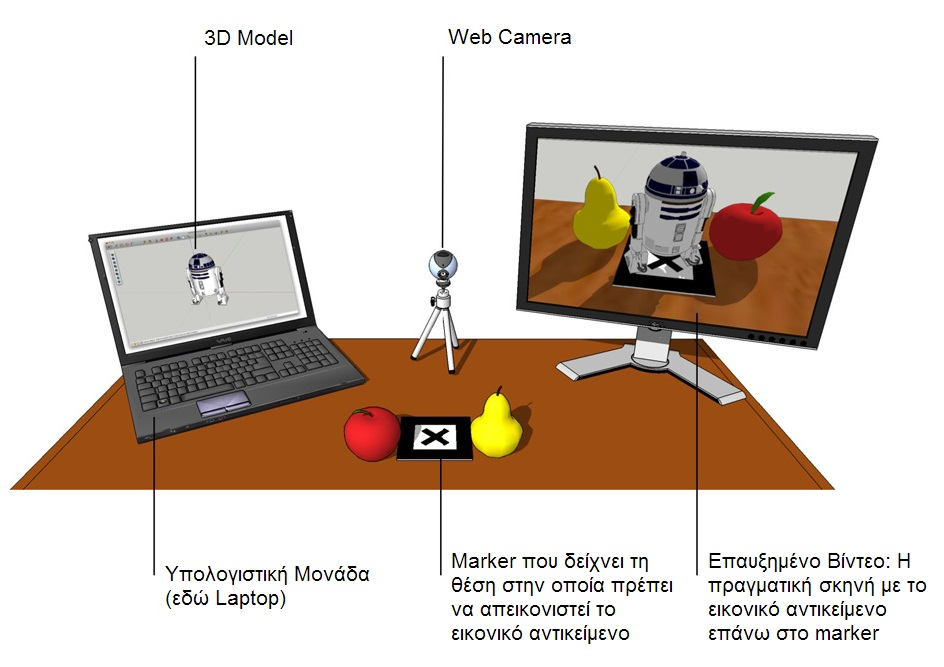
\includegraphics[scale=0.3, angle=0]{Files/Figures/ar_system_example.jpg}
    \caption[Παράδειγμα εγκατάστασης ενός συστήματος επαυξημένης πραγματικότητας ]{ Παράδειγμα εγκατάστασης ενός συστήματος επαυξημένης πραγματικότητας \cite{ar_example}}
    \label{fig:ar_example}
\end{figure}


Η κύρια διαδικασία για τη σωστή λειτουργία ενός συστήματος επαυξημένης πραγματκότητας έχει να κάνει με το κομμάτι της ανίχνευσης. Το κομμάτι αυτό ασχολείται με τον υπολογισμό της σχετικής πόζας της κάμερας σε πραγματικό χρόνο. Με τον όρο πόζα (pose) περιγράφουμε τους 6 βαθμούς ελευθερίας της τοποθεσίας ενός αντικειμένου, δηλαδή τη θέση του στον τρισδιάστατο χώρο και τον προσανατολισμό στον τριασδιάστατο χώρο.

Η διαδικασία της ανίχνευσης είναι αυτή που επιτρέπει την προσθήκη εικονικών αντικειμένων σε μία πραγματική σκηνή.
Η βασική διαφορά σε σύγκριση με άλλα εργαλεία επεξεργασίας εικόνας παρατηρείται στο γεγονός ότι στην επαυξημένη πραγματικότητα τα εικονικά αντικείμενα μετακινούνται και περιστρέφονται σε 3 διαστάσεις αντί για 2 όπως γίνεται συνήθως σε εικόνες.  Ο απλούστερος τρόπος εκτίμησης της πόζας είναι η χρήση δεικτών (markers). 
Ωστόσο, το μαθηματικό μοντέλο ( προβολική γεωμετρία) πίσω από τις μεθόδους υπολογισμού της πόζας είναι το ίδιο. 

Παρόμοια προβλήματα βελτιστοποίησης διαμορφώνονται σε διαφορετικές μεθόδους υπολογισμού της πόζας και λύνονται με τις ίδιες μεθόδους βελτιστοποίησης.  
Μπορούμε να θεωρήσουμε ότι οι markers είναι ένας ειδικός τύπος χαρακτηριστικού και επομένως μπορούμε να ορίσουμε μεθόδους με βάση την ανίχνευση markers και μετέπειτα μεθόδους με βάση την ανίχνευση χαρακτηριστικών, καθώς και υβριδικές μεθόδους. Στη συγκεκριμένη διπλωματική εργασία θα επικεντρωθούμε σε συστήματα επαυξημένης πραγματικότητας που βασίζονται σε markers.

Συνήθως η καταγραφή της εικόνας δεν είναι σημαντικό κομμάτι στην επαυξημένη πραγματικότητα. Συνήθως χρησιμοποιούνται έτοιμες βιβλιοθήκες για το σκοπό αυτό,

Τα εργαλεία και οι βιβλιοθήκες επαυξημένης πραγματικότητας παρέχουν υποστήριξη για την καταγραφή εικόνας και βίντεο. Η διαδικασία τηςα απεικόνισης ζωγραφίζει την εικονική εικόνα πάνω στην εικόνα του βίντεο. Στα γραφικά υπολογιστών, η εικονική σκηνή προβάλλεται πάνω στο επίπεδο της εικόνας χρησιμοποιώντας μία εικονική κάμερα και αυτή η προβολή απεικονίζεται στο τέλος. 

Απαιτείται ουσιαστικά η χρήση μίας εικονικής κάμερας που είναι παρόμοια με τη πραγματική κάμερα του συστήματος. Με αυτό τον τρόπο τα εικονικά αντικείμενα προβάλλονται στη σκηνή με τον ίδιο τρόπο με τον οποίο θα προβάλλονταν πραγματικά αντικείμενα και το αποτέλεσμα είναι γεωμετρικά πειστικό. Για να μπορέσουμε να μιμηθούμε τις ιδιότητες της πραγματικής κάμερας, το σύστημα πρέπει να ξέρει τα οπτικά χαρακτηριστικά της κάμερας. Η διαδικασία κατά την οποία προσδιορίζονται αυτά τα χαρακτηριστικά ονομάζεται βαθμονόμηση κάμερας.

Η βαθμονόμηση της κάμερας μπορεί να είναι μέρος του συστήματος επαυξημένης πραγματικότητας ή ξεχωριστή διαδικασία. Πολλές βιβλιοθήκες παρέχουν εργαλεία βαθμονόμησης, όπως για παράδειγμα οι βιβλιοθήκες ArUco, ALVAR, ARToolkit.


Ωστόσο για τη διαδικασία της βαθμονόμησης μπορούν να χρησιμοποιηθούν και τρίτα εργαλεία βιβλιοθηκών όπως το Matlab ή η OpenCV. 

Στην εργασία αυτή αφού περιγράψουμε τη διαδικασία της βαθμονόμησης, θεωρούμε ότ έχουμε πάντα μία σωστά βαθμονομημένη κάμερα για την ανάπτυξη της εφαρμογής μας.

Η ποικιλία των συσκευών οι οποίες υποστηρίζουν συστήματα επαυξημένης πραγματικότητας είναι μεγάλη και περιλαμβάνει σταθερούς και φορητούς υπολογιστές, tablets, κινητά και άλλες υπολογιστικές μονάδες. Ανάλογα με την εφαρμογή, μπορεί να αξιοποιηθεί η ενσωματωμένη κάμερα της συσκευής, μία απλή USC κάμερα, μία Firewire κάμερα ή μία ψηφιακή κάμερα. Μπορεί επίσης να χρησιμοποιηθεί μία συσκευή απεικόνισης που προσαρτάται στο κεφάλι του χρήστη(HMD), μία συσκευή απεικόνισης οπτικής τεχνολογίας ή η ίδια η οθόνη της υπολογιστικής μονάδας. Επίσης μπορεί το σύστημα να προβάλλει την επαυξημένη σκηνή στον πραγματικό κόσμο\cite{jones2013illumiroom} ή να χρησιμοποιηθεί μια στερεοσκοπική συσκευή απεικόνισης. Η κατάλληλη εγκατάσταση εξαρτάται από την εφαρμογή και το περιβάλλον στο οποίο αναπτύσσεται.








%vallino
Ο συνδυασμός πραγματικών και εικονικών εικόνων σε μία συγχωνευμένη εικόνα παρουσιάζει τεχνικές δυσκολίες για τους σχεδιαστές εφαρμογών επαυξημένης πραγματικότητας.  Το ερώτημα, στο οποίο καλούνται να απαντήσουν, έχει να κάνει με το πώς θα πραγματοποιηθεί η συνένωση των δύο εικόνων.




Η τεχνολογία θέασης αποτελεί ένα από τα βασικότερα συστατικά στοιχεία των συστημάτων επαυξημένης πραγματικότητας. Οι τεχνολογίες θέασης των συστημάτων επαυξημένης πραγματικότητας μπορούν να χωριστούν σε τρεις κύριες κατηγορίες [4], [45]. Αυτές είναι οι συσκευές προσάρτησης στο κεφάλι ή σε μέρος του κεφαλιού του χρήστη, οι φορητές συσκευές χειρός και οι συσκευές απεικόνισης των συστημάτων χωρικής επαυξημένης πραγματικότητας (Spatial Augmented Reality - SAR). Στην ενότητα αυτή παρουσιάζονται τα τρία αυτά είδη τεχνολογιών θέασης της επαυξημένης σκηνής \cite{azuma1997} \cite{Vallino1998}  \cite{azuma2001} \cite{Krevelen2010} .









-Head-Worn Displays (HWDs)
Οι συσκευές αυτές, γνωστές ως Head-Worn Displays (HWD) ή Head-Attached Displays, φοριούνται στο κεφάλι του χρήστη ή σε κάποιο μέρος του κεφαλιού. Στις παρακάτω παραγράφους περιγράφονται οι κυριότερες κατηγορίες των συσκευών αυτών.

-Head-Mounted Displays (HMDs)

%eftekhari
Στην επαυξημένη πραγματικότητα υπάρχουν δύο βασικές κατηγορίες συστημάτων απεικόνισης που αξιοποιούν τα HMDs ως μέσο για την οπτική διεπαφή. 

 Optical see-through HMDs require that the user has the ability to see-through the display medium to the surrounding real world. This is achieved by placing partially transmissive optical combiners in front of the eyes. Each system has particular advantages and disadvantages pertained by their conceptual design and it is necessary to consider the trade-o s between the two before opting to implement one as part of an AR system. It should also be noted that non-immersive HMDs may be monocular or binocular (see gure 2.3), distinctions between the these must also be considered when choosing to design an optical based system, [48]. Optical approaches are simpler and cheaper than WoW. The world is seen directly through the optical combiners, meaning there is only one video stream to be concerned with. In see-through systems the only information available about the users head location comes from a head tracker. The WoW approach however, provides additional information via streaming digitised video image computer generated images for which virtual imagery can be analogically or digitally overlaid onto. This is achieved by using a technique called chroma-keying often observed in movies with video special e ects. The background of the computer graphic image is set to a speci c color, say green, which none of the virtual objects use. Then the combining step replaces all green areas with the corresponding parts from the video of the real world. This has the e ect of superimposing the virtual objects over the real world. The computational expense of executing chroma-keying techniques in real time can lead to poor performance. This can present a problem of temporal distortion when real and virtual images are not properly synchronised. Thus, using post-processing computation on video streams results in time delays of a few nanoseconds with optical systems to tens of milliseconds with WoW systems. Angular resolution describes the resolving power of any image forming device. This includes; microscopes, telescopes, optical displays, cameras or the naked eye. Unaided the human eye can resolve to the power of around 100 micro metres. Though the eye recieves data from a broad range of about 200 degrees, the acuity over most of the range is poor. High resolution images must fall on the fovea and as a result acute vision is limited to around 15 degrees. The fovea is located in the centre of the retina and is 2.5 - 3 mm in diameter. Since the fovea provides the most detailed and colourful information, the eye ball is constantly moving, enabling light from the object of primary interest to fall on this region. The actual perception of a scene is constructed by the eye-brain


%vallino
To increase the sense of presence other display technologies are needed. Head-mounted displays (HMD) are widely used in virtual reality systems. Augmented reality researchers work with two types of HMD. These two types are called video see-through and optical see-through. The “see-through” designation comes from the need for the user to be able to see the real world view that is immediately in front of him even when wearing the HMD. The standard HMD used in virtual reality work gives the user complete visual isolation from the surrounding environment. Since the display is visually isolating the system must use video cameras that are aligned with the display to obtain the view of the real world. A diagram of a video see-through system is shown in Figure 16. Video see-through is really the same architecture as the monitor-based display except that now the user has a heightened sense of immersion in the display. Some experiments with a video see-through system have been done as part of our work (Section 4.5.4). Figure 17 shows the configuration of two video cameras mounted on an HMD.






Ένα σύστημα Head-Mounted Display (HMD) είναι μία συσκευή που προσαρτάται στο κεφάλι του χρήστη και συνδυάζει την εικόνα του πραγματικού κόσμου με εικονικά αντικείμενα, μέσω χρήσης οπτικής ή βίντεο τεχνολογίας [5], [54].

-optical see through
Τα οπτικά συστήματα παρουσίασης προσαρτημένα στο κεφάλι του χρήστη (optical seethrough HMDs) τοποθετούν μπροστά από τα μάτια του «οπτικούς συνδυαστές» (συνήθως ημιδιαπερατά και ημιανακλαστικά κάτοπτρα), που του επιτρέπουν να δει τόσο το πραγματικό περιβάλλον γύρω του, όσο και τις παραγόμενες από υπολογιστή εικόνες που ανακλούνται μέσω των κατόπτρων από τις οθόνες που είναι προσαρτημένες στο κεφάλι του (βλ. Εικόνα 1-24).


%valino
The optical see-through HMD (Manhart, Malcolm et al. 1993) eliminates the video channel that is looking at the real scene. Instead, as shown in Figure 18, the merging of real world and virtual augmentation is done optically in front of the user. This technology is similar to heads up displays (HUD) that commonly appear in military airplane cockpits and recently some experimental automobiles. In this case, the optical merging of the two images is done on the head mounted display, rather than the cockpit window or auto windshield, prompting the nickname of “HUD on a head”.

%krevelen
Optical see-through techniques with beam-splitting holographic
optical elements (HOEs) may be applied in
head-worn displays, hand-held displays, and spatial setups
where the AR overlay is mirrored either from a planar screen
or through a curved screen.
These displays not only leave the real-world resolution in
tact, they also have the advantage of being cheaper, safer, and
parallax-free (no eye-offset due to camera positioning). Optical
techniques are safer because users can still see when
power fails, making this an ideal technique for military and
medical purposes. However, other input devices such as
cameras are required for interaction and registration. Also,
combining the virtual objects holographically through
transparent mirrors and lenses creates disadvantages as it
reduces brightness and contrast of both the images and the
real-world perception, making this technique less suited for
outdoor use. The all-important field-of-view is limited for
this technique and may cause clipping of virtual images at the
edges of the mirrors or lenses. Finally, occlusion (or mediation)
of real objects is difficult because their light is always
combined with the virtual image. Kiyokawa et al. [90] solved
this problem for head-worn displays by adding an opaque
overlay using an LCD panel with pixels that opacify areas to
be occluded.
Virtual retinal displays or retinal scanning displays (RSDs)
solve the problems of low brightness and low field-of-view in
(head-worn) optical see-through displays. A low-power laser
draws a virtual image directly onto the retina which yields
high brightness and a wide field-of-view. RSD quality is not
limited by the size of pixels but only by diffraction and aberrations
in the light source, making (very) high resolutions
possible as well. Together with their low power consumption
these displays are well-suited for extended outdoor use. Still
under development at Washington University and funded by
MicroVision7 and the U.S. military, current RSDs are mostly
monochrome (red only) and monocular (single-eye) displays.
Schowengerdt et al. [143] already developed a full-colour,
binocular version with dynamic refocus to accommodate the
eyes (Fig. 5) that is promised to be low-cost and light-weight

%mcdonald
The optical alternative for HMD systems is a technology that combines real objects with virtual ones in a different way than the video see-through systems. As shown in Figure 2.6, the optical see-through system does not use video input at all. The real-world component of the augmentation is simply the user’s actual view of the environment. The user sees an augmented scene through the use of optical combiners, which add the graphics output to the real view. The advantage of an optical see-through system is that the user is viewing the actual environment, as opposed to a video representation of it. Since the user views the actual scene the virtual component is the only possible source of lag. And for the same reason the scene quality of direct view of the world is superior to a video representation. Therefore using a see-through system eliminates the problem of system lag and improves the quality of view of the augmented scene. The disadvantage of this type of system is that there is no video input signal to help with the registration process. This has the potential to reduce registration accuracy if the chosen head tracking method is not accurate. The other disadvantage to the optical seethrough system is that the quality of the virtual augmentation is usually low. As seen in figure 2.7, the small optical combiner in front of the eye is a low-resolution display. This weakness restricts the freedom of graphical output. If an AR application requires very high detailed virtual objects, a video see-through or monitor-based system would probably be required.

%malik
The other popular HMD configuration for augmented reality is the optical see-through display system, as depicted in Figure 1.6. In this setup, the user is able to view the real world through a semi-transparent display, while virtual objects are merged into the scene optically in front of the user’s eyes based on the user’s current position. Thus when users move their heads, the virtual objects maintain their positions in the world as if they were actually part of the real environment. Unlike the video see-through displays, these HMDs do not exhibit the limited resolutions and delays when depicting the real world. However, the quality of the virtual objects will still be limited by the processing speed and graphical capabilities of the augmentation system. Therefore, creating convincing augmentations becomes somewhat difficult since the real world will appear naturally while the virtual objects will appear pixilated. The other major disadvantage with optical see-through displays is their lack of single frame captures of the real world, since no camera is present in the default hardware setup. Thus position sensors within the HMD are the only facility through which pose information can be extracted for registration purposes1. Some researchers have proposed hybrid solutions that combine position sensors with video cameras in order to improve the pose estimation; Section 2.4 discusses these hybrid solutions in more detail.


-video see through
Τα HMDs που χρησιμοποιούν βίντεο τεχνολογία (video see-through HMDs), συνδυάζουν ένα «κλειστό» HMD (closed-view HMD1) και μία ή δύο βιντεοκάμερες προσαρτημένες στο κεφάλι του χρήστη, οι οποίες του παρέχουν μία θέα του πραγματικού κόσμου. Το βίντεο από τις κάμερες αυτές και οι παραγόμενες εικονικές σκηνές συνδυάζονται μεταξύ τους και το αποτέλεσμα στέλνεται στις οθόνες που βρίσκονται μπροστά από τα μάτια του χρήστη στο closed-view HMD (βλ. Εικόνα 1-25). Το HMD αναφέρεται και ως Helmet-Mounted Display (βλ. Εικόνα 1-26, κέντρο) και προσαρμόζεται στο κράνος του χρήστη κυρίως για εφαρμογές στην αεροπορία και ιδιαίτερα σε μαχητικά αεροσκάφη [55]. Νεότερα από τα HMDs είναι τα προσαρτημένα επί κεφαλής συστήματα παρουσίασης μέσω προβολής, γνωστά ως Head-Mounted Projective Displays (HMPDs) (βλ. Εικόνα 1-26, δεξιά). Τα κυριότερα μέρη των συστημάτων αυτών είναι ένας μικροσκοπικός προβολικός φακός στερεωμένος στο κεφάλι του χρήστη και οπισθοανακλαστικές (retroreflective) επιφάνειες που τοποθετούνται μπροστά από αυτόν. Οι ακτίνες φωτός που προσπίπτουν στις επιφάνειες αυτές εκτρέπονται προς την κατεύθυνση πρόσπτωσής τους και δεν διαχέονται, όπως συμβαίνει με τα συμβατικά προβολικά συστήματα, με αποτέλεσμα να παράγουν φωτεινότερες εικόνες [56], [57], [58].


%krevelen
Besides being the cheapest and easiest to implement, this
display technique offers the following advantages. Since
reality is digitised, it is easier to mediate or remove objects
from reality. This includes removing or replacing fiducial
markers or placeholders with virtual objects (see for instance
Fig. 7 and 22). Also, brightness and contrast of virtual objects
are matched easily with the real environment. Evaluating the
light conditions of a static outdoor scene is of importance
when the computer generated content has to blend in
smoothly and a novel approach is developed by Liu et al.
[101].
The digitised images allow tracking of head movement for
better registration. It also becomes possible to match perception
delays of the real and virtual. Disadvantages of video
see-through include a low resolution of reality, a limited
field-of-view (although this can easily be increased), and user
disorientation due to a parallax (eye-offset) due to the camera‟
s positioning at a distance from the viewer‟s true eye
location, causing significant adjustment effort for the viewer
[35]. This problem was solved at the MR Lab by aligning the
video capture [153]. A final drawback is the focus distance of
this technique which is fixed in most display types, providing
poor eye accommodation. Some head-mounted setups can
however move the display (or a lens in front of it) to cover a
range of .25 meters to infinity within .3 seconds [150]. Like
the parallax problem, biocular displays (where both eyes see
the same image) cause significantly more discomfort than
monocular or binocular displays, both in eye strain and fatigue
[53].

%mc donald
Σε ένα σύστημα video see-through, a head-mounted camera is used in conjunction with a head mounted tracker to gather the necessary scene input. The viewpoint position is given to the graphics system to render the virtual objects in their proper position. The real world scene is captured by the video camera, combined with the graphics output, and displayed to the user through the head-mounted monitor system. Figure 2.4 outlines this HMD technology system. As shown in Figure 2.5, a user of this type of HMD is presented with all aspects of the scene through the head-mounted monitor. This means the real scene must be merged with the graphics output in order to display the augmented scene to the user. This merging process adds delays to the system. The amount of system delay directly translates into lag time seen by the user, which reduces the user’s feeling of presence. This is a disadvantage to the video see-through technology that cannot be avoided, but can be minimized. The advantage of this type of system is that while gathering the real scene through video, information about the scene can be extracted. This capability can assist in the process of tracking the head position and thus leading to a more accurate registration. Another advantage to this type of system is that the video display is typically high-resolution. This means that there is the potential to render highly detailed virtual objects in combination with the input video. An alternative to having the video input is the optical see-through technology.


%malik
In order to increase the sense of immersion in virtual reality systems, head-mounted displays (HMD) that fully encompass the user’s view are commonly employed. There are two popular methods to bring HMDs into the augmented reality environment. Figure 1.5 shows a schematic for a video see-through augmented reality system. In this configuration, the user does not see the real world directly, but instead only sees what the computer system displays on the tiny monitors inside the HMD. The difference between this and a virtual reality HMD is the addition of video cameras to capture images of the real world. While this configuration is almost identical to the monitor-based technology in terms of functionality, the use of a stereo camera pair (two cameras) allows the HMD to provide a different image to each eye, thereby increasing the realism and immersion that the augmented world can provide. Like the monitor-based setup, the video seethrough display is prone to visual lags due to the capture, processing, augmentation, and rendering of each video frame. Additionally, a large offset between the cameras and the user’s eyes can further reduce the sense of immersion, since everything in the captured scenes will be shifted higher or lower than where they should actually be (with respect to the user’s actual eye level).

%tzionas
Μπορούμε να δημιουργήσουμε ένα video see-through AR σύστημα είτε με τη βοήθεια ενός closed view see-through HMD14  και μίας head mounted κάμερας είτε με τη βοήθεια φορητών συσκευών σε συνδυασμό με μία κάμερα (βλ εικόνα 7). Ο χρήστης δεν αντιλαμβάνεται τον πραγματικό κόςμο απευθείας με τα μάτια του, αλλά με διαμεσολάβηση μίας κάμερας και μίας οθόνης που τον προβάλει. Ταυτόχρονα, σε κάθε frame επικάθονται στην εικόνα του πραγματικου κόσμου και εικονικές πληροφορίες, και το τελικό αποτέλεσμα προβάλλεται σε μία οθόνη στο ύψος των ματιών.




Monitor-based Display
%malik
The simplest approach is a monitor-based display, as depicted in Figure 1.4. The video camera continuously captures individual frames of the real world and feeds each one into the augmentation system. Virtual objects are then merged into the frame, and this final merged image is what users ultimately see on a standard desktop monitor. The advantage of this display technology is its simplicity and affordability, since a consumer-level PC and USB or FireWire video camera is all that is required. Additionally, by processing each frame individually, the augmentation system can use vision-based approaches to extract pose (position and orientation) information about the user for registration purposes (by tracking features or patterns, for example). However this simplicity comes at the expense of immersion. Clearly, viewing the real world through a small desktop monitor limits the realism and mobility of the augmented world. Additionally, since each frame from the camera must be processed by the augmentation system, there is a potential delay from the time the image is captured to when the user actually sees the final augmented image. Finally, the quality of the imagery is limited by the resolution of the camera.

%valino
Monitor-based or WoW (window on the world) (see gure 2.3) refer to a display system where the user views the world in real time via a capture-display device. This usually involves a webcam which feeds the images to small LCD screens placed close to the eyes;


\section{Pinhole Camera Model}
%TO ΜΟΝΤΕΛΟ ΚΑΜΕΡΑΣ ΑΠΟ ΑΛΛΗ ΕΡΓΑΣΙΑ-

\subsection{Βαθμονόμηση}
%Η ΔΙΑΔΙΚΑΣΙΑ ΒΑΘΜΟΝΟΜΗΣΗΣ ΚΑΙ ΓΕΝΙΚΑ Η ΘΕΩΡΙΑ ΑΠΟ ΠΙΣΩ(ΤΟ ΠΩς ΓΙΝΕΤΑΙ ΣΤΟ ΚΕΦΑΛΑΙΟ 4)

\subsection{Intrinsics}
\subsection{Extrinsics}




\section{Tracking}
%ΓΕΝΙΚΑ ΑΝΑΦΕΡΕ ΤΙ ΕΙΝΑΙ ΤΟ TRACKING
Augmented reality presents information in a correct real world context. In order to do this, the system needs to know where the user is and what the user is looking at. Normally, the user explores the environment through a display that portrays the image of the camera together with augmented information. Thus in practice, the system needs to determine the location and orientation of the camera. With a calibrated camera, the system is then able to render virtual objects in the correct place. The term tracking means calculating the relative pose (location and orientation) of a camera in real time. It is one of the fundamental components of augmented reality.

Researchers in computer vision, robotics and photogrammetry have developed a considerable number of different tracking methods. People can divide these methods based on the equipment used in sensor tracking methods, visual tracking methods and hybrid methods. Since in most augmented reality setups the camera is already part of the system, visual tracking methods are of special interest in AR.

We will concentrate on them first and discuss sensor and hybrid tracking methods later in Chapter 5. In visual tracking, the system deduces the pose of the camera based on observations of what it sees. In an unknown environment, this is challenging; it takes some time to collect enough data to be able to deduce the pose and then the calculated pose estimation easily drifts over time. As the environment is unknown to the system, the system selects the orientation of the coordinate axis at random, which may be inconvenient for the user. In addition, it is impossible to deduce the correct scale solely based on visual observations. One solution to overcome these challenges is to add an easily detectable predefined sign in the environment and use computer vision techniques to detect it. A marker is such a sign or image that a computer system can detect from a video image using image processing, pattern recognition and computer vision techniques (e.g. right image in Figure 23). Once detected, it then defines both the correct scale and pose of the camera. This approach is called marker-based tracking, and it is widely used in AR. Other approaches for visual tracking are feature-based and model-based methods, which we will discuss later in Chapter 5. In model-based tracking, the system has a model of the scene or part of the scene (e.g. a CAD model). It compares visual observations with the model and finds the best match, which then defines the pose. In feature-based tracking, the system detects optical features in the images and learns the environment based on observations of movements between frames. Even though mainstream visual tracking research leans towards feature-based tracking, feature tracking and marker-based tracking are mutually non-exclusive. In fact, marker-based methods often outperform feature-based methods in certain occasions (as we will rationalise later in Section 4.4.1.), and marker-based systems are still widely used for visual tracking in augmented and mixed reality (e.g. [68–70]. The popularity of marker-based systems is also partly explained by the fact that they are easy to implement and that good and well-known marker-based toolkits are available (e.g. ARToolKit [64], ALVAR [19], ARTag [71]). Toolkits provide a good base for starting AR application development. Apart from that, markers provide the correct scale and convenient coordinate frames (Figure 23) as previously mentioned. In addition, they may encode information or at least have an identity. This enables a system to attach certain objects or interactions to the markers. In marker-based tracking, the system needs to detect the marker, identify it and then calculate the pose. In this chapter, we focus on marker detection and pose estimation. We talk more about different marker types and identifying and decoding markers in Chapter 4. We go through the pipeline of the marker detection procedure, considering commonly used black and white square markers. Section 3.1 gives an overview of the detection process and most of the steps and methods presented here serve for detecting other types of markers and other tracking methods as well.

In Section 3.2, we explain how camera pose is estimated using the four corner
points of a marker. At the end of this chapter in Section 3.3, we discuss multimarker
setups that improve the tracking system.

\subsection{Marker Tracking}
%MONO FIDUCIAL MARKER TRACKING

%siltanen
A good marker is easily and reliably detectable under all circumstances. Differences in luminance (brightness) are more easily detected than differences in chrominance (colour) using machine vision techniques. [72] This is due to the poor automatic white balance of the cameras: the colours register incorrectly, and an object may change its colour in the image depending on what else is in the view, for example. Furthermore, the lighting changes the perceived colours of the objects and therefore colour detection is challenging. Naturally, the more contrast in the luminance the more easily objects are detected. In this sense, black and white markers are optimal. The system should also be able to calculate the pose of the camera using the detected marker. Four known points are sufficient to calculate the pose of a camera uniquely [72] and the simplest shape to acquire them is a square. In addition, the locations of the corner points are relatively robust, as they can be estimated as intersections of edge lines. Therefore, many of the marker systems use black and white square markers. This is also why we first go through the marker detection process considering such markers. We cover other marker types later in the Chapter 4.

%des siltanen gia marker detection procedure



%---
The commonly used technique to perform tracking nowadays is based on optical devices (conventional web camera, ToF, structured light) applying image processing and computer vision algorithms. 

The simplest tracking method in AR is by using fiducial markers, Figure 1, its basic working process consists on a tracking algorithm that performs a series of image processing tasks over each frame of a video sequence in order to detect where a marker is, and a registration which correlates a virtual object to the physical marker\cite{krevelen2010}. It consists on threshold the image and look for the edges using a scanline search. With the known edges of the marker, it fits a rectangle by finding the corners based on the maximum diagonals between the points in the edges, this is done with the purpose of delimit the rectangle where a pattern is recognized and matched against a pattern stored in memory. Once we recognize the pattern, the pose of the marker is estimated by calculating the rotation and translation parameters relative to the camera. This action is done using a transformation matrix formed with the angles (rotation) and translation vectors (translation). In other words, we want to know the coordinates of the marker with respect of the camera coordinates using this transformation points called extrinsic parameters (varies according of the movement of the camera) while the intrinsic parameters are used to move from the camera coordinates to the image coordinates and are fixed on the camera by calibration; these are the focal distance, scale parameters and (x,y) center coordinates of the projection image. With the position of the marker detected, a virtual model is placed on the same position of the image coordinate relatively to the marker. This gives the impression that the virtual object is stick to the marker and the process is called registration. The resulting image is shown in a display in which the user see the virtual object superposed over the real world. The process is done dynamically and fast enough to give the impression of real-virtual world correlation. It is not computationally expensive but the marker must be easily recognizable, i.e. the lighting conditions must be favourable and it should not be partially occluded, otherwise the recognition can fail.

    
\subsection{Markerless Tracking}
%SLAM-PTAM,FEATURE DETECTION,SURF ETC
%πολύ λίγα λόγια-περιληπτικά



\section{Αναγνώριση Χειρονομιών}
%ΓΕΝΙΚΑ ΓΙΑ ΤΗΝ ΑΝΑΓΝΩΡΙΣΗ ΧΕΙΡΟΝΟΜΙΩΝ ΚΑΙ ΤΗΝ ΚΟΙΝΩΝΙΚΗ ΑΠΟΔΟΧΗ ΚΑΙ ΤΗ ΧΡΗΣΙΜΟΤΗΤΑ ΣΕ ΕΦΑΡΜΟΓΕΣ


%Από εργασία μου δερματά

H αναγνώριση χειρονομιών είναι η διαδικασία κατά την οποία οι χειρονομίες οι οποίες γίνονται από τον χρήστη αναγνωρίζονται από έναν δέκτη. Η αναγνώριση και η ερμηνεία των χειρονομιών απαιτεί από τη μηχανή την ικανότητα να μετρήσει τις δυναμικές ή στατικές παραμορφώσεις του χεριού, του βραχίονα ή ακόμα και άλλων μερών του ανθρωπίνου σώματος, τα οποία συμμετέχουν στην κίνηση.

Σε κάθε σύστημα αναγνώρισης χειρονομιών το πρώτο στάδιο είναι η συλλογή δεδομένων από τον χρήστη.Οι πρώτες συσκευές συλλογής δεδομένων βασιζόντουσαν στη χρήση data gloves και καλωδίων, πράγμα που εμπόδιζε την φυσικότητα στην αλληλεπίδραση του χρήστη.Οι σημερινές προσεγγίσεις αξιοποιούν την χρήση βιντεοκάμερων και τεχνικών υπολογιστικής όρασης που καταγράφουν το αντικείμενο και με τεχνικές αναγνώρισης αναλύουν και ερμηνεύουν τις χειρονομίες.

Πολλές και ποικίλες είναι οι προσεγγίσεις των ερευνητών στην αναγνώριση των χειρονομιών.Αυτά που διαφέρουν σε κάθε προσέγγιση είναι ο τρόπος με τον οποίο κάθε ερευνητής κατάφερε να συλλέξει δεδομένα και οι τεχνικές επεξεργασίας εικόνας που εφάρμοσε για να εξάγει χαρακτηριστικά.

Οι νοηματικές χειρονομίες μπορούν να είναι πολύ σύνθετες, περιέχοντας ταυτόχρονες κινήσεις διάφορων σημείων, ωστόσο πρέπει να περιγραφούν στον υπολογιστή με τρόπο απλό και σαφή.

Pinch It is defined as the movement of expansion and contraction of a nger spread. It has been used for different purposes depending on target applications, e.g. the zooming metaphor by contracting and expanding, scaling or picking. It resembles a grabbing or picking action and offers natural signal to select or move an object in an interactive system and due to the nature of the thumb and index ngers, the pinch grabbing is precise and has high performance.


Human interaction with computer technology has for many years been a machine-centric form of communication. It has relied on the user’s ability to conform to interface strategies that better suit the technology than the user. As the use of computer technology spreads, the physical and expressive limitations of current interaction methods are increasingly counter-productive. Current interface technology such as the mouse and keyboard associated with desktop computers has become ubiquitous in mainstream computing. This role is based on application interface technology that has been used for decades. As the application domain expands, this technology will reveal its performance inhibitions. In an effort to overcome the barrier associated with current interface solutions, much research is being done in the domain of gesture recognition. Because gesture recognition is a natural form of human expression, it seems reasonable to apply it to the communication channel of Human-Computer Interaction (HCI). Several techniques for capturing gesture have been proposed [OKA02, ULHA01, CROW95]. Gesture interpretation for HCI requires the measurability of hand, arm and body configurations. Initial methods were attempted to directly measure hand movements using glove-based strategies. These methods required that the user be attached to the computer through the connecting cables. This restricts the user significantly in their environment.

Overcoming this contact-based interpretation requires the inference-based methods of computer vision. As processor power continues to rise, the once complex algorithms of the field are becoming available as real-time applications. Most computer vision-based gesture recognition strategies focus on static hand gestures known as postures. However, it has been argued that the motion within gesture communication conveys as much meaning as the postures themselves. Examples include global hand motion and isolated fingertip motion analysis. The interpretation of gesture can be broken down into three phases: modeling, analysis and recognition. Gesture modeling involves the schematic description of a gesture system that accounts for its known or inferred properties. Gesture analysis involves the computation of the model parameters based on detected image features captured by the camera. The recognition phase involves the classification of gestures based on the computed model parameters. These phases are outlined in figure 2.12.

Although much research has been done in the field of gesture recognition, HCI interaction involving accurate, real-time interpretation is a long way off. The key to simplifying the domain of human gesture possibilities is to construct a gesture model which clearly describes the sub-domain of gesture that will be classified by the associated system.



To determine an appropriate model for a given HCI system, the application must be clearly defined. Simple gesture requirements result in simple gesture models. Likewise, complex gesture interpretation, involves defining a complex model.

Gesture is defined as the use of body and motion as a form of expression and social interaction. This interaction must be interpreted for communication to be successful. Gesture interpretation is considered a psychological issue, which plays a role in the taxonomy of the varying types of human gesture. Figure 2.13 outlines one such taxonomy.

It is crucial for any gesture recognition system to distinguish between the higher level classifications such as gesture versus unintentional movements and manipulation versus communicative. It has been suggested that the temporal domain of human gesture, for example, can help classify a gesture from unintentional movement. The temporal aspect of gesture has three phases: preparation, nucleus, and retraction [PAVL97]. The preparation phase involves the preparatory movement of the body from its rest position. The nucleus phase involves a definite form of body, while the retraction phase describes the return of the body to its rest position. The preparation and retraction phase are characterized by rapid motion, whereas the nucleus phase shows relatively slow motion. Some measurable stray from these temporal properties could indicate unintentional movement as opposed to gestures in the classification process. Two forms of modeling are being explored; appearance and 3D model-based modeling. Appearance-based modeling deals with the direct interpretation of gesture from images using templates. Image content features such as contours, edges, moments and even fingertips can form a basis for parameter extraction with respect to the gesture model chosen. Three-dimensional model-based modeling is used to describe motion and posture in order to then infer the gesture information. Volumetric models are visually descriptive, but are complex to interpret using computer vision. Skeletal models describe joint angles which can be used to infer posture and track motion.


\subsection{Αναγνώριση Blob}
%ΤΙ ΕΙΝΑΙ Η ΑΝΑΓΝΩΡΙΣΗ BLOB


\subsection{Αναγνώριση Χειρονομίας Τσιμπήματος}
%ANALYΣΕ ΤΟ PINCH, ΠΩΣ ΓΙΝΕΤΑΙ, ΓΙΑΤΙ ΕΙΝΑΙ ΕΥΚΟΛΟ,ΠΟΥ ΧΡΗΣΙΜΟΠΟΙΕΙΤΑΙ, ΠΩΣ ΑΝΙΧΝΕΥΕΤΑΙ(WILSON,ETC)

%wang-popovi


Pinching has been shown to be an effective gesture for “clicking”
in 3D space. Hilliges and colleagues use a single depth
camera to detect pinches above a table top [9]. Benko and
Wilson [4] track pinches using an infrared camera above a
projector. Wilson uses a webcam to detect pinches above
the keyboard [26]. However, all three approaches rely on
a single-view pinch detection technique that suffers from occlusions,
restricting the hand orientations that can be tracked.
A unique feature of our approach is the use of two widebaseline
viewpoints. Our two-view approach resolves occlusions
from one view using information from the other, enabling
robust gesture (e.g. pinch) detection. Our contribution
is independent of the particular type of camera used (depth
or RGB).
%--

Successful gesture recognition requires clear classification of the model parameters. This process can be difficult when attempting feature extraction schemes that rely on complex computer vision techniques. For example, contours can be misinterpreted when used for the recognition of gesture so their use is usually restricted to tracking. On the other hand, slight changes in hand rotation while presenting the same posture can be interpreted as different postures using geometric moments. Temporal variance is an important issue that needs to be studied in more detail. For example, hand clapping should be recognized properly regardless if it is done slowly or quickly. Hidden Markov Models (HMMs) have shown promise in distinguishing gesture in the presence of duration and variation changes

Another recognition approach is to use motion history images (MHIs) or temporal templates. Motion templates accumulate the motion history of a sequence of visual images into a single two-dimensional image. Each MHI is parameterized by the time history window that was used for its computation. Multiple templates with varying history window times are gathered to allow time duration invariance. This process is computationally simple, but recognition problems can stem from the presence of artifacts in the images when auxiliary motions are present. Although it seems that 3D model-based approaches can capture the richest set of hand gestures in HCI, the applications that use such methods are rarely real-time. The most widely used gesture recognition approaches use appearance-based models. Current applications in the field of hand gesture related to HCI are attempting to replace the keyboard and mouse hardware with gesture recognition. Exciting possibilities with helping physically-challenged individuals and the manipulation of virtual objects are being explored.



%\section{Διαδραστική Επαυξημένη Πραγματικότητα}
%OTI ΔΕΝ ΕΙΠΑΜΕ ΣΤΗΝ ΕΙΣΑΓΩΓΗ ΓΙΑ AR, ΚΥΡΙΩΣ ΑΝΑΦΟΡΑ ΕΡΓΑΣΙΩΝ ΠΟΥ ΑΣΧΟΛΟΥΝΤΑΙ ΜΕ INTERACTION OF VIRTUAL OBJECTS, KAI MEΘΟΔΟΥΣ ΠΟΥ ΧΡΗΣΙΜΟΠΟΙΟΥΝΤΑΙ, ΓΙΑΤΙ ΕΙΝΑΙ ΧΡΗΣΙΜΗ Η ΑΛΛΗΛΕΠΙΔΡΑΣΗ ΣΤΟ ar


\section{Σχετικές Ερευνητικές Εργασίες}
%ΑΝΑΦΕΡΕ ΠΑΡΟΜΟΙΕΣ ΕΡΓΑΣΙΕΣ ΓΙΑ GESTURE INTERACTION, AR TABLETOP GAMING, KAI AZUMA CLASSICS ETC.
%ΠΕΣ ΣΙΓΟΥΡΑ ΓΙΑ ΠΑΡΟΜΟΙΑ ΣΚΑΚΙΑ ΣΤΟ ΤΕΛΟΣ
%ΨΑΧΝΟΝΤΑΣ ΣΕ PAPERS ΑΝΑΦΕΡΕ ΠΑΡΟΜΟΙΕΣ ΕΡΓΑΣΙΕΣ ΝΑ ΕΧΟΥΝ ΣΧΕΣΗ ΜΕ GESTURE RECOGNITION FOR AR, VIRTUAL OBJECT MANIPULATION, AR TABLETOP GAMES
Σε προηγούμενες ερευνητικές εργασίες, παρουσιάστηκαν διαφορετικές προσεγγίσεις για την κατανόηση των δυνατοτήτων που προσφέρουν οι χειρονομίες στην αλληλεπίδραση με εικονικά αντικείμενα σε ένα περιβάλλον επαυξημένης πραγματικότητας. Επιπλέον, σε βιβλιογραφικές αναφορές μπορούμε να εντοπίσουμε τις δυνατότητες της επαυξημένης πραγματικότητας στον χώρο της ψυχαγωγίας και συγκεκριμένα των βιντεοπαιχνιδιών, τις βασικές έννοιες της αλληλεπίδρασης μεσω χειρονομιών και της ρεαλιστικής απεικόνισης εικονικών αντικειμένων.


%thomas-cie-apps of ar gaming
Augmented reality chess games have been implemented on previous works. One approach
[1] used a handheld pen prop with a marker cube on top of it in order to interact with the
chess pieces. As the writers admit, the tracking of interaction props was inaccurate and slow
to provide unencumbered and natural use. Another one[2] used nger tracking techniques that
allow gestural interaction with the chess pieces. In this approach, manipulation of virtual objects
is possible using grab and release gestures, as well as image processing techniques to detect hand
gestures, using a single camera. The nger tracker that is implemented is using a hands 3D
model that can determine enough information to robustly track the position, orientation and
pose of the users index nger. However, this solution resorts to using a marked glove with
retro-re
ective spheres on top of the forengers joints, something that may disturb users and is
denitely not a natural way to interact with content. Other approaches utilize mobile markers
that correspond to a specic type of chess piece and users had to move the markers to different
positions of a chessboard in order to play the chess game. Of course this would take quite an
amount of effort to correctly print and create the congurable chessboard and is really similar
to just using a real chessboard with real chess pieces.


Η εφαρμογή AR2Hockey ήταν ένα από τα πρώτα βιντεοπαιχνίδια στο χώρο της επαυξημένης πραγματικότητας[Ohshima et al. 1998]. Στο συγκεκριμένο παιχνίδια, χρησιμοποιοιείται τεχνολογία optical see-through HMD display για 2 παίκτες. The game is played on a standard table with landmarks. The landmarks allow for a hybrid optical tracking and the Polhemus’ Fastrack. The game basically supports the traditional form of air hockey, but replaces the physical pucks with virtual ones. As an extension to this,Mueller et al. developed an AR remote version of air hockey [Mueller et al. 2006]. Two remote physical air hockey tables, one for each player, provide the playing surface for the game. There is a video conferencing display across the middle of each table providing a real-time video feed of the other player. What makes this game different is that the users play with physical pucks. Once a puck is hit across the table, it is caught with a mechanism under the video conference display. The mechanism then automatically shoots the puck back in response to the shot from the other player. The game of pool (or billiards) has been investigated by a number of researchers as an application domain for AR. Jebara et al. developed the first mobile AR pool system [Jebara et al. 1997]. This is an HMDbased AR game, for which many of the first algorithms for image processing and physics engines for pool-based games were developed. This game served as a trainer for the end user by displaying AR information on the correct cue placement. Each of these games supports a physical gaming interface, adding to the evidence that AR incorporates both the physical and virtual worlds. AR2Hockey was a very early AR game, and as such required more expensive display and tracking equipment; but the price for both these forms of hardware has fallen dramatically. The Jebara et al. pool system also required a large structure, the pool table, to play the game upon. This system also incorporates a tutoring system for the players, including suggestions for shots.


A number of AR card games have been developed: Billinghurst et al. created an ARToolkit memory game, where the users flip physical cards [Billinghurst et al. 2000]. When a card is flipped over, a 3D graphic is displayed. The cards interact with each other by playing an animation when there is a match between the cards. This was the first AR game developed with the ARToolkit. Diaz et al. created a variant which employed hand gestures as the means of interaction [Diaz et al. 2006]. They used special cards to enable the system to sense card flipping by embedding Hall effect switches in the cards. BattleBoard is another example of a tabletop AR card game [Andersen et al. 2004]. This is an ARToolkit fiducial marker-based AR system which attaches virtual game pieces to the markers. One player employs an HMD with a camera and the second player views the game through a monitor. Battles are fought when pieces come in close proximity to each other, and thus activate AR animations. The Billinghurst et al. card game was designed for a public demonstration at an ACM SIGGraph conference with quick gameplay. BattleBoard employs a similar technology to the Billinghurst et al. card game, but BattleBoard’s design is more advanced, and is similar to a duelling card game. The Tankwar game was developed for more extended gameplay, investigating how AR could be employed for games with a more traditional time span.


%interaction in ar games
A drama-based game, Fac¸ade, was extended into an HMD AR version, AR Fac¸ade [Dow et al. 2007a, 2006, 2007b]. This game is a major break from traditional AR gaming ideas developed previously. This is a complex, real-life, role-playing game; very much like interactive theatre. Originally, the game was played on a traditional workstation; AR Fac¸ade is played on a HMD with a mobile backpack system, with gestures and voice as the main forms of interaction. The authors constructed virtual and physical representations of many of the game objects, such as walls and furniture, in an apartment. Objects that were manipulated by both the virtual characters and the physical players were presented as AR objects to the game player in the HMD. Due to the large area the game is played in a large area with an IS1200 tracking system. A Wizard of Oz method was employed to support user interactions to make formore robust gesture and speech processing systems during user studies. The authors found this form of interaction engaging for the user, but more research is required

%playstation app with board and monitor for AR
Το βιντεοπαιχνίδι Eye of Judgement της πλατφόρμας Sony PS3 είναι ένα βιντεοπαιχνίδι επαυξημένης πραγματικότητας σε τρίτο πρόσωπο, που περιλαμβάνει μία ψηφιακή βιντεοκάμερα η οποία καταγράφει το ταμπλό του παιχνιδιού και απεικονίζει μία επαυξημένη του έκδοση στην τηλεόραση. Αυτός ο τύπος παιχνιδιού απαιτεί από τους χρήστες να επικεντρώνουν την προσοχή τους τόσο στο πραγματικό ταμπλό, όσο και στην έκδοση που παρουσιάζεται στην οθόνη. Μόλις οι κάρτες του παιχνιδιού τοποθετηθούν πάνω στο ταμπλό, δρουν ως καθοδηγητικοί δείκτες(markers) για τον εντοπισμό τεράτων επαυξημένης πραγματικότητας και τα κομμάτια του παιχνιδιού απεικονίζονται επάνω τους. Η μηχανή παιχνιδιών αναλαμβάνει τα τρισδιάστατα γραφικά των καρτών μόλις εντοπιστούν. Το παιχνιδί αυτό, ήταν ένα από τα πρώτα εμπορικά βιντεοπαιχνίδια επαυξημένης πραγματικότητας που κυκλοφόρησαν στην αγορά που επέτρεπε τη χρήση καθογητητικών δεικτών (fiducial markers).


%Εργασίες με σκάκι ή pinch gestures για χειρισμό εικονικών αντικειμένων 
Οι Dorfmuller-Ulhaas και Schmalstieg δημιούργησαν ένα σύστημα οπτικής ανίχνευσης δακτύλων, με απώτερο σκοπό την αφαίρεση των ενοχλητικών καλωδίων κατά τη διάρκεια της αλληλεπίδρασης με τα εικονικά αντικείμενα. Μάλιστα, η τεχνολογίας που ανέπτυξαν, παρουσιάστηκε μέσα από μία επαυξημένη έκδοση ενός πολύ γνωστού παιχνιδιού, που δεν είναι άλλο από το σκάκι. [Dorfmuller-Ulhaas and Schmalstieg 2001].

%vale kai mobile collaborative ar chess


%wang,popovi
RELATED WORK
Many methods have been proposed for markerless or gloveless
hand tracking, but they are either too slow for interactive
applications, e.g. [24, 7], or the range of poses that they can
detect do not permit the precise selection required in CAD
applications, e.g. [14, 13, 20]. In comparison, our system
achieves bimanual 6-DOF pose estimation at interactive rates
and reliably detects poses suited for discrete selection such as
pinching and pointing.
Glove tracking has been proposed to ease and speed up the
problem of hand tracking, e.g. [27, 25]. However, gloves are
a significant drawback if one wants to also use the keyboard
and mouse. Users may be reluctant to put on a glove when
switching from a 2D task such as menu navigation to a 3D
task such as object assembly. Wearing a glove may also become
uncomfortable during long work sessions.


%krevelen
Besides registering virtual data with the user‟s real world
perception, the system needs to provide some kind of interface
with both virtual and real objects. Our technological
advancing society needs new ways of interfacing with both
the physical and digital world to enable people to engage in
those environments [67]. 
WIMP (windows, icons, menus, and pointing), as the
conventional desktop UI metaphor is referred to, does not
apply that well to AR systems. Not only is interaction required
with six degrees of freedom (6DOF) rather than 2D, the use of conventional devices like a mouse and keyboard
are cumbersome to wear and reduce the AR experience.
Like in WIMP UIs, AR interfaces have to support selecting,
positioning, and rotating of virtual objects, drawing
paths or trajectories, assigning quantitative values (quantification)
and text input. However as a general UI principle,
AR interaction also includes the selection, annotation, and,
possibly, direct manipulation of physical objects. This
computing paradigm is still a challenge [20].




In stead of using hand-worn trackers, hand movement may
also be tracked visually, leaving the hands unencumbered. A
head-worn or collar-mounted camera pointed at the user‟s
hands can be used for gesture recognition. Through gesture
recognition, an AR could automatically draw up reports of
activities [105]. For 3D interaction, UbiHand uses
wrist-mounted cameras enable gesture recognition [14],
while the Mobile Augmented Reality Interface Sign Interpretation Language 16 [16] recognises hand gestures on a
virtual keyboard displayed on the user‟s hand (Fig. 12). A
simple hand gesture using the Handy AR system can also be
used for the initialization of markerless tracking, which estimates
a camera pose from a user‟s outstretched hand [97].
Cameras are also useful to record and document the user‟s
view, e.g. for providing a live video feed for teleconferencing,
for informing a remote expert about the findings of AR
field-workers, or simply for documenting and storing everything
that is taking place in front of the mobile AR system
user.
Common in indoor virtual or augmented environments is
the use of additional orientation and position trackers to
provide 6DOF hand tracking for manipulating virtual objects.
For outdoor environments, Foxlin and Harrington [60] experimented
with ultrasonic tracking of finger-worn acoustic
emitters using three head-worn microphones




Immersed in an environment containing virtual information, the user is left with few mechanisms for interacting with the virtual augmentations. The use of hardware devices [VEIG02] can be physically restrictive given the special freedom goals of Augmented Reality. Interaction with virtual augmentation through a physical mediator such as a touch screen [ULHA01] is becoming a common practice. An interesting alternative is the use of natural human gestures to communicate directly with the environment. Gesture recognition has been explored mainly for the purpose of communicative interaction. Gesture systems have explored many aspects of hand gesture including three-dimensional hand posture [HEAP96] and fingertip motion [OKA02, ULHA01, CROW95]. The system presented in this chapter attempts to bridge these two fields of study by describing a hand gesture system that is used for manipulative interaction with the virtual augmentation. Although natural human gestures are too complex to recognize in realtime, simple gesture models can be defined to allow a practical interactive medium for real-time Augmented Reality systems.

\section{Προκλήσεις και προβλήματα}
%ΣΥΓΧΡΟΝΑ ΠΡΟΒΛΗΜΑΤΑ ΣΤΟ AR

%ziegler
2.3.5 State of the Art Recent tracking systems produced very good results for indoor applications. Predominantly, they use hybrid approaches and work within a limited range (cp. [ZDB08, HF04, ABB+01]). According to Zhou et al.[ZDB08] current tracking systems consist of two stages. The first stage is dedicated to either learning and training or feature extraction. The second stage takes care of the tracking itself, using the knowledge gained through training or the features that have been extracted. The first stage usually requires the most computational resources, if the system uses a learning algorithm. Using a learning stage can reduce the resources the on-line tracking needs, enabling the system to work in real time. 2.3.5.1 Limitations and Challenges Even though tracking systems are accurate enough to achieve good results, the environments they work in are usually restricted not only to being indoors but also to being known in advance[ABB+01]. Dynamical adaption to unknown environments still poses a challenge. Complex scenes are challenging for real-time 3D tracking as is the motion of target objects[ZDB08]. Coping with rapid camera movements is difficult as resulting motion-blur hinders the re-observation of features. Rapid and unpredictable changes, that may occur in outdoor environments, constrain tracking results[HF04]. Especially illumination changes, which often and repeatedly occur outdoors, complicate the tracking process[ZDB08]. Basically all changes which cannot be controlled or anticipated are hard to handle. Some systems feature automatic reinitialisation, but the recovery of the camera pose, when the tracking has failed, cannot be achieved easily[ZDB08]. It is limited to applications which possess enough knowledge about the environment or which do not solely rely on vision-based tracking. 2.3.5.2 Trends Current research features many tracking approaches. Coping with unknown outdoor environments is an important topic. One way researchers are trying to achieve that is by further investigating hybrid approaches. As the growing number of publications during the past years indicate, Mobile AR becomes more and more popular among researches[SW07, WRM+08]. The growing computational resources of mobile devices present novel possibilities. The number of commercial applications from which users can choose continually rises. Among them are Layar9, Nokia Point & Find10, Twitter AR11 and Virus Killer 36012. Building a reference presentation of the environment while tracking is a popular trend, research focusing especially on Simultaneous Localisation and Mapping (SLAM)[CGKM07, DRMS07, KM09]. Such systems usually require a high amount of computational resources. However, through certain restrictions, SLAM works on a mobile phone, too, as has recently been shown by the work of Klein and Murray[KM09]. Instead of using as many features as possible and hoping that some of the chosen features provide robust tracking, researchers try to find methods to detect only suitable and useful features in the first place[ZDB08, ST94]. Researchers try to find ways of making initialisation processes automatic[SKSK07]. Focusing on model-based tracking is popular as well[FL07, WS07]. Last but not least, ubiquitous tracking, that is tracking acquired by forming a dense network of sensors that enables tracking everywhere, seems to be achievable in the near future[HPK+07].


%--
Μία από τις μεγαλύτερες προκλήσεις με τις οποίες έρχονται αντιμέτωποι οι δημιουργοί εφαρμογών επαυξημένης πραγματικότητας είναι η σωστή τοποθέτηση του εικονικού αντικειμένου εντός του πραγματικού περιβάλλοντος, έτσι ώστε η συνθετική πληροφορία να δίνει την εντύπωση ότι ανήκει σε αυτό. Η διαδικασία αυτή είναι γνωστή ως registration (γεωαναφορά). Η σωστή συγχώνευση και ευθυγράμμιση των δύο κόσμων – του φυσικού και του παραγόμενου από υπολογιστή – είναι κύρια προϋπόθεση για την εκπλήρωση του στόχου των εφαρμογών επαυξημένης πραγματικότητας, ενώ λάθη ή ανακρίβειες στην τοποθέτηση του εικονικού αντικειμένου θα έχουν ως αποτέλεσμα να χαθεί η ψευδαίσθηση ότι οι δύο κόσμοι συνυπάρχουν [3]. Πολλές εφαρμογές, μάλιστα, όπως για παράδειγμα στην ιατρική, απαιτούν ακριβή γεωαναφορά και δεν είναι επιτρεπτά λάθη και αστοχίες. Για τη σωστή γεωαναφορά, απαραίτητη προϋπόθεση είναι η πρότερη ανίχνευση της θέσης και του προσανατολισμού της κάμερας – και γενικά της συσκευής μέσω της οποίας επαυξάνεται η πραγματικότητα – ή του κεφαλιού του χρήστη (π.χ. σε εφαρμογή με HMD). Η διαδικασία αυτή είναι γνωστή ως tracking (ανίχνευση), απαντά στα ερωτήματα: πού βρίσκεται ο χρήστης, πού εστιάζεται το ενδιαφέρον του και πού πρέπει να παρουσιαστεί το εικονικό αντικείμενο [72] και συνεπώς η σωστή και ακριβής, ανάλογα με την εφαρμογή διεκπεραίωσή της είναι κρίσιμη για τη δημιουργία πειστικών εφαρμογών επαυξημένης πραγματικότητας. Για την επίτευξη των τελευταίων, η ανίχνευση πρέπει πρακτικά να διεξάγεται σε πραγματικό χρόνο, δηλαδή η εκτίμηση της θέσης να γίνεται σε χιλιοστά του δευτερολέπτου, καθώς επίσης και να είναι εύρωστη, δηλαδή να δίνει ικανοποιητικά αποτελέσματα κάτω από ποικίλες συνθήκες, όπως για παράδειγμα σε μεταβαλλόμενο φωτισμό [68]. Υπάρχουν πολλές μέθοδοι ανίχνευσης 6 βαθμών ελευθερίας (6DOF tracking), όπως το μηχανικό tracking, τεχνική που υιοθετήθηκε και από το πρώτο σύστημα επαυξημένης πραγματικότητας του Sutherland, το υπερηχητικό tracking και το οπτικό tracking. Υπάρχουν και άλλες που υπολογίζουν μόνο θέση ή προσανατολισμό, όπως για παράδειγμα το tracking που βασίζεται σε πληροφορίες μόνο από GPS ή μόνο από γυροσκόπια [15]. Για εφαρμογές που απαιτούν ακριβή γεωαναφορά, ωστόσο, απαιτείται ακριβές στιγμιαίο 6DOF tracking υπό οποιεσδήποτε συνθήκες. Επειδή η τέλεια ανίχνευση είναι – τουλάχιστον προς το παρόν – ανέφικτη, εξαιτίας των χρονικών καθυστερήσεων ή και των περιορισμών λόγω ακριβείας, κύρια πρόκληση αποτελεί η εύρεση της μεθόδου ανίχνευσης που είναι ιδανική για τη συγκεκριμένη κάθε φορά εφαρμογή [73]. Υπάρχει ένας ακόμη αριθμός προκλήσεων που συνδέονται με το πρόβλημα της ανίχνευσης και τοποθέτησης του εικονικού αντικειμένου εντός του φυσικού περιβάλλοντος [4], η κυριότερη από τις οποίες είναι οι αποκρύψεις (occlusion). Σύμφωνα με την τελευταία, πρέπει να επιτυγχάνεται η πλήρης ή μερική απόκρυψη του εικονικού αντικειμένου όταν κάποιο άλλο αντικείμενο του πραγματικού περιβάλλοντος τοποθετείται μπροστά από αυτό και το κρύβει, πλήρως ή μερικώς. Άλλη δυσκολία στις εφαρμογές επαυξημένης πραγματικότητας, σχετική με την οπτική ανίχνευση, είναι η μη εστιασμένη κάμερα στο marker ή στο πρότυπο που πρέπει να αναγνωριστεί για την επαύξηση της πραγματικότητας, γεγονός το οποίο μπορεί να οδηγήσει στη μη αναγνώρισή του, ή σε λάθη στην τοποθέτηση του εικονικού αντικειμένου, λόγω της χαμηλότερης ακρίβειας με την οποία αποδίδεται. Μία ακόμη πρόκληση, συγγενική με την οπτική ανίχνευση (visual tracking), είναι ο μη ομοιόμορφος φωτισμός, λόγω του οποίου ένα marker μπορεί να συσκοτιστεί σε κάποια τμήματά του και να μην αναγνωρίζεται από το πρόγραμμα ή να αναγνωρίζεται ως διαφορετικό marker. Όμοια, λόγω μεταβαλλόμενου φωτισμού, υπάρχει η πιθανότητα μη αναγνώρισης της εικόνας που έχει οριστεί ως πρότυπο. Τέλος, η θαμπάδα που μπορεί να προκληθεί λόγω γρήγορης κίνησης της κάμερας – κυρίως μίας κινητής συσκευής – είναι ένας ακόμα παράγοντας που δύναται να δυσκολέψει τη σωστή επαύξηση της πραγματικής σκηνής. Ένα κύριο στοιχείο των εφαρμογών επαυξημένης πραγματικότητας είναι η απεικόνιση του εικονικού αντικειμένου στην πραγματική σκηνή, δηλαδή η δημιουργία της συνθετικής επαυξημένης σκηνής, σε πραγματικό χρόνο (real-time rendering). Η φύση κάποιων εφαρμογών απαιτεί οι γραφικές πληροφορίες να ενσωματώνονται στο φυσικό περιβάλλον με τέτοιο τρόπο ώστε ο παρατηρητής να μην μπορεί να ξεχωρίσει ποιο είναι το πραγματικό και ποιο το εικονικό. Στις εφαρμογές αυτές, εκτός από το σωστό και ακριβές tracking και registration, απαιτείται ταυτόχρονα και φωτορεαλιστικό rendering, με σωστή σκίαση και φωτισμό του εικονικού αντικειμένου και οποιαδήποτε άλλη αυτόματη από το λογισμικό επεξεργασία πραγματικού χρόνου αυτό συνεπάγεται [6]. Καθοριστικό στοιχείο στη βελτίωση της ποιότητας του rendering αποτελεί η ικανότητα της εφαρμογής να λαμβάνει και να αξιοποιεί πληροφορία για το φωτισμό του περιβάλλοντος και την ανάκλαση [3]. Ένα ακόμη βασικό στοιχείο των εφαρμογών επαυξημένης πραγματικότητας είναι, όπως έχει ήδη αναφερθεί, η τεχνολογία θέασης, η οποία ταυτόχρονα αποτελεί και μία πρόκληση, καθώς η βελτίωσή της, ανάλογα με τις απαιτήσεις της εκάστοτε εφαρμογής, μπορεί να συντελέσει σε μεγαλύτερη αποδοχή της τεχνολογίας αυτής από το κοινό. Πράγματι, είναι πολύ πιο βολικό και «γνώριμο» στον άνθρωπο να φορέσει γυαλιά ή φακούς που θα επαυξήσουν την πραγματικότητά του σε σχέση με κάποια βαριά και μεγάλη συσκευή που προσαρτάται στο κεφάλι του (HMD ή HMPD). Εκτός από τέτοιου είδους περιορισμούς, που οφείλονται στον ανθρώπινο παράγοντα και για τους οποίους γίνονται σήμερα πολλές προσπάθειες βελτίωσης, υφίστανται και άλλες προκλήσεις σχετικές με την τεχνολογία θέασης της επαυξημένης πραγματικότητας [6], όπως είναι για παράδειγμα οι οπτικοί περιορισμοί λόγω του περιορισμένου οπτικού πεδίου του χρήστη, καθώς και οι τεχνικοί περιορισμοί, όπως η περιορισμένη ανάλυση και διάφοροι άλλοι παράγοντες. Εκτός των παραπάνω σημαντικών προκλήσεων με τις οποίες έρχονται αντιμέτωπες οι εφαρμογές επαυξημένης πραγματικότητας, υπάρχουν και άλλα τεχνικά ζητήματα σχετικά με αυτές, όπως είναι η αλληλεπίδραση του χρήστη με την εικονική πληροφορία, γεγονός το οποίο θα του δώσει την αίσθηση της πλήρους ενσωμάτωσης στο συνθετικό αυτό κόσμο, που συνδυάζει το πραγματικό με το εικονικό. Τέλος, οι δημιουργοί των εφαρμογών επαυξημένης πραγματικότητας πρέπει να δίνουν σημασία και στο πλήθος των εικονικών πληροφοριών που υπερτίθενται στο πραγματικό περιβάλλον του χρήστη, έτσι ώστε αυτό να μην εμποδίζει το χρήστη από τη θέαση του φυσικού κόσμου, αλλά ούτε και να είναι ανεπαρκές.
 
%krevelen

AR faces technical challenges regarding for example binocular
(stereo) view, high resolution, colour depth, luminance,
contrast, field of view, and focus depth. However,
before AR becomes accepted as part of user‟s everyday life,
just like mobile phones and personal digital assistants
(PDAs), issues regarding intuitive interfaces, costs, weight,
power usage, ergonomics, and appearance must also be addressed.
A number of limitations, some of which have been
mentioned earlier, are categorised here.

-Portability and outdoor use
Most mobile AR systems mentioned in this survey are
cumbersome, requiring a heavy backpack to carry the PC,
sensors, display, batteries, and everything else. Connections
between all the devices must be able to withstand outdoor use,
including weather and shock, but universal serial bus (USB)
connectors are known to fail easily. However, recent developments
in mobile technology like cell phones and PDAs
are bridging the gap towards mobile AR.
Optical and video see-through displays are usually unsuited
for outdoor use due to low brightness, contrast, resolution,
and field of view. However, recently developed at
MicroVision, laser-powered displays offer a new dimension
in head-mounted and hand-held displays that overcomes this
problem.
Most portable computers have only one CPU which limits
the amount of visual and hybrid tracking. More generally,
consumer operating systems are not suited for real-time
computing, while specialised real-time operating systems
don‟t have the drivers to support the sensors and graphics in
modern hardware.

-Tracking and (auto)calibration
Tracking in unprepared environments remains a challenge
but hybrid approaches are becoming small enough to be added to mobile phones or PDAs. Calibration of these devices
is still complicated and extensive, but this may be
solved through calibration-free or auto-calibrating approaches
that minimise set-up requirements. The latter use
redundant sensor information to automatically measure and
compensate for changing calibration parameters [19].
Latency A large source of dynamic registration errors are
system delays [19]. Techniques like precalculation, temporal
stream matching (in video see-through such as live broadcasts),
and prediction of future viewpoints may solve some
delay. System latency can also be scheduled to reduce errors
through careful system design, and pre-rendered images may
be shifted at the last instant to compensate for pan-tilt motions.
Similarly, image warping may correct delays in 6DOF
motion (both translation and rotation).

-Depth perception
One difficult registration problem is accurate depth perception.
Stereoscopic displays help, but additional problems
including accommodation-vergence conflicts or low resolution
and dim displays cause object to appear further away
than they should be [52]. Correct occlusion ameliorates some
depth problems [138], as does consistent registration for
different eyepoint locations [158].
In early video see-through systems with a parallax, users
need to adapt to vertical displaced viewpoints. In an experiment
by Biocca and Rolland [35], subjects exhibit a large
overshoot in a depth-pointing task after removing the HMD.

-Overload and over-reliance
Aside from technical challenges, the user interface must
also follow some guidelines as not to overload the user with
information while also preventing the user to overly rely on
the AR system such that important cues from the environment
are missed [156]. At BMW, Bengler and Passaro [29] use
guidelines for AR system design in cars, including orientation
on the driving task, no moving or obstructing imagery,
add only information that improves driving performance,
avoid side effects like tunnel vision and cognitive capture,
and only use information that does not distract, intrude or
disturb given different situations.

-Social acceptance
Getting people to use AR may be more challenging than
expected, and many factors play a role in social acceptance of
AR ranging from unobtrusive fashionable appearance
(gloves, helmets, etc.) to privacy concerns. For instance,
Accenture‟s Assistant (Fig. 14) blinks a light when it records
for the sole purpose of alerting the person who is being recorded.
These fundamental issues must be addressed before
AR is widely accepted [73].

%---
The diversity of AR platforms, devices, tools and applications is stunning. Overall,
augmented reality is a pronounced visualisation method, which is used in many
application areas. It is especially advantageous in on-site real-time visualisations
of database information and for purposes where there is a need to enhance the
3D perceptive skills of the user. Augmented reality enables natural interactions
and is a good tool to create interactive games and enhance user experience in
other areas as well. In this work, we aim to give a thorough overview of the whole
field, whilst concentrating on the fundamental issues of single-camera visual augmented
reality.


In conclusion, the augmented reality application developer needs to take into consideration several different issues: technical, application and other issues affecting the user experience. The main technological issues relate directly to the definition of augmented reality (real-time, interactive, 3D, combining real and virtual). Application issues arise from the ease of creating AR applications. Other important issues relate to user experience. The main technological issues in augmented reality are �� performance �� interaction �� alignment.

The main application issues are �� content creation �� authoring. Other important issues affecting the user experience are �� visual perception �� user interface �� devices �� power consumption. Next, we review what we mean by these issues and how they affect the usability and user experience of an AR application. An augmented reality system needs to be able to perform in real-time. Otherwise, the system may augment old or flawed information, or the augmentation may not correspond to the current state of the environment. Performance issues are characteristic to all AR algorithm and application development. Research results from other fields (e.g. image processing) are not directly applicable to AR. For instance, traditional image inpainting methods do not fulfil the real-time requirement, and therefore they cannot be used for diminished reality as such (see Section 6.2). Performance is an issue especially in mobile environment where the processing power and memory are limited. The user should be able to interact with the system naturally. The usability and the user experience are disturbed if the interaction is unnatural. The interaction needs to be natural in the user interface level as we discussed in the Section 7.1. The same holds true at the application level; the interaction between the real world objects and virtual objects needs to be smooth as well. Application needs to adapt virtual elements according to real scene, as for example in our interior design application where the user was able to adjust virtual lights easily according to real ones (see Section 6.1.3). At times, the application needs to remove existing objects virtually to be able to augment virtual objects on the same place. We discussed in Section 6.2 how to handle this kind of interaction with diminished reality. The camera calibration needs to be correct and the tracking needs to be accurate. Otherwise, the augmented data is shifted in the real environment: the virtual overlay is in the wrong place or it flutters. People find this alignment error annoying. In Chapter 3, we concentrated on marker-based approaches for accurate tracking, and in Chapter 4, on alternative tracking methods, mainly feature-based tracking and hybrid tracking methods. In addition, Appendix C gives an overview of camera calibration. The content creation is also an important aspect of application development. An application can visualise information from a database (e.g. in augmented assembly) or provide textual information (e.g. in AR browsers). Sometimes the information in database is in unsuitable format and format conversion is needed. In addition, when no database is available someone needs to create the content. Furthermore, if nice graphics are required, they need to be created to the approboth mobile environments and high quality visualisation. Besides content creation, authoring is a big application issue as we discussed in Section 7.4. Creation of AR applications should be brought to a non-expert nonprogramming level, where users can combine objects, interactions and events at a conceptual level. Visual perception should support the purpose of the application as we discussed in Chapter 6. Some applications require (photo-)realistic rendering, other applications benefit from focus and content -type highlighting of augmented objects. The user should be able to concentrate on the task, and the visual perception should sustain the task, without distracting the user. The user interface should be, as always, easy to use and intuitive. It should support the task at hand and make the user experience smooth as discussed in Section 7.1. The AR application should run on the appropriate device; mobile applications on lightweight devices, high-end visualisations on larger good-quality monitors. Furthermore, the terminal device should be taken into account already at the application design stage. There is no point in implementing computationally intensive methods on mobile phones if the application would then run on a slow frame rate. Devices often play very important role in the development process. The diversity of mobile platforms is perhaps the main obstacle for wider use of mobile AR applications. Applications need to be ported mostly to each platform separately, which deprives resources from application development. Furthermore, mobile devices are an ideal platform for consumer applications; they are equipped with cameras and new models with various additional sensors; people carry them with them all the time. Likewise, in special applications where an expert operates the system, it is feasible to invest in special devices such as HMDs, 3D displays, additional sensors, etc. if they support the task. One more aspect that significantly affects user experience is power consumption. Many applications require the user to be able to move freely, and thus wireless devices are optimal and then battery life plays a big role. A mobile application that discharges the battery in 15 minutes is unrealistic. We once tested a HMD where the camera ran out of batteries in less than two hours. The user had to change the batteries often, which was annoying especially as the camera and projector were wired to a computer anyway. It is hard to imagine this kind of setup in practical use, e.g. in a factory. In conclusion, the most important issue of augmented reality application development is the user experience, which is affected by all technological, application and other issues.


Η ποικιλομορφία συσκευών, εργαλείων και εφαρμογών επαυξημένης πραγματικότητας είναι εντυπωσιακή. Γενικά, η τεχνολογία της επαυξημένης πραγματικότητας είναι μια μέθοδος απεικόνισης που μπορεί να χρησιμοποιηθεί σε πολλές εφαρμογές, ενώ παράλληλα επιτρέπει φυσικές αλληλεπιδράσεις και είναι ένα καλό εργαλείο ανάπτυξης διαδραστικών βιντεοπαιχνιδιών που μπορεί να ενισχύσει την εμπειρία που βιώνουν οι χρήστες. Σε αυτή την εργασία, στοχεύουμε στη δημιουργία μιας μεθόδου που προσφέρει απλό και γρήγορο χειρισμό των εικονικών αντικειμένων. Οι αλγόριθμοι που αναπτύσσονται, εξετάζονται και αξιολογούνται υλοποιώντας ένα βιντεοπαιχνίδι επαυξημένης πραγματικότητας του γνωστού επιτραπέζιου παιχνιδιού, του σκακιού.


